\chapter{Results and Evaluation} \label{chap:results}

In this chapter, I will present the results and evaluation of the experimental setup from Chapter \ref{chap:exp_setup}. In this evaluation, I will consider the following configurations:

\begin{itemize}
    \item \textbf{Vortex}\footnote{https://github.com/EECS-NTNU/vortex-ntnu/tree/ntnu\_main} is the baseline version of \Gls{vortex} as presented at MICRO'21~\cite{vortex}.
    \item \textbf{FGTO}\footnote{\label{fn:gh_larsmaur}https://github.com/EECS-NTNU/vortex-ntnu/tree/ntnu\_main\_larsmaur} is the configuration implementing ready scheduling, and all the frontend changes, i.e. \acrshort{bpr}, \acrshort{nss} and stall-prediction. The \acrshort{gto} scheduling algorithm is used for both the warp and instruction scheduler.
    \item \textbf{FRRR}\footnotemark[2] is the configuration implementing ready scheduling, and all the frontend changes, i.e. \acrshort{bpr}, \acrshort{nss} and stall-prediction. The \acrshort{lrr} scheduling algorithm is used for both the warp and instruction scheduler.
\end{itemize}

\section{CPI Stack Overview}

\begin{figure}
    \centering
    \makebox[\textwidth][c]{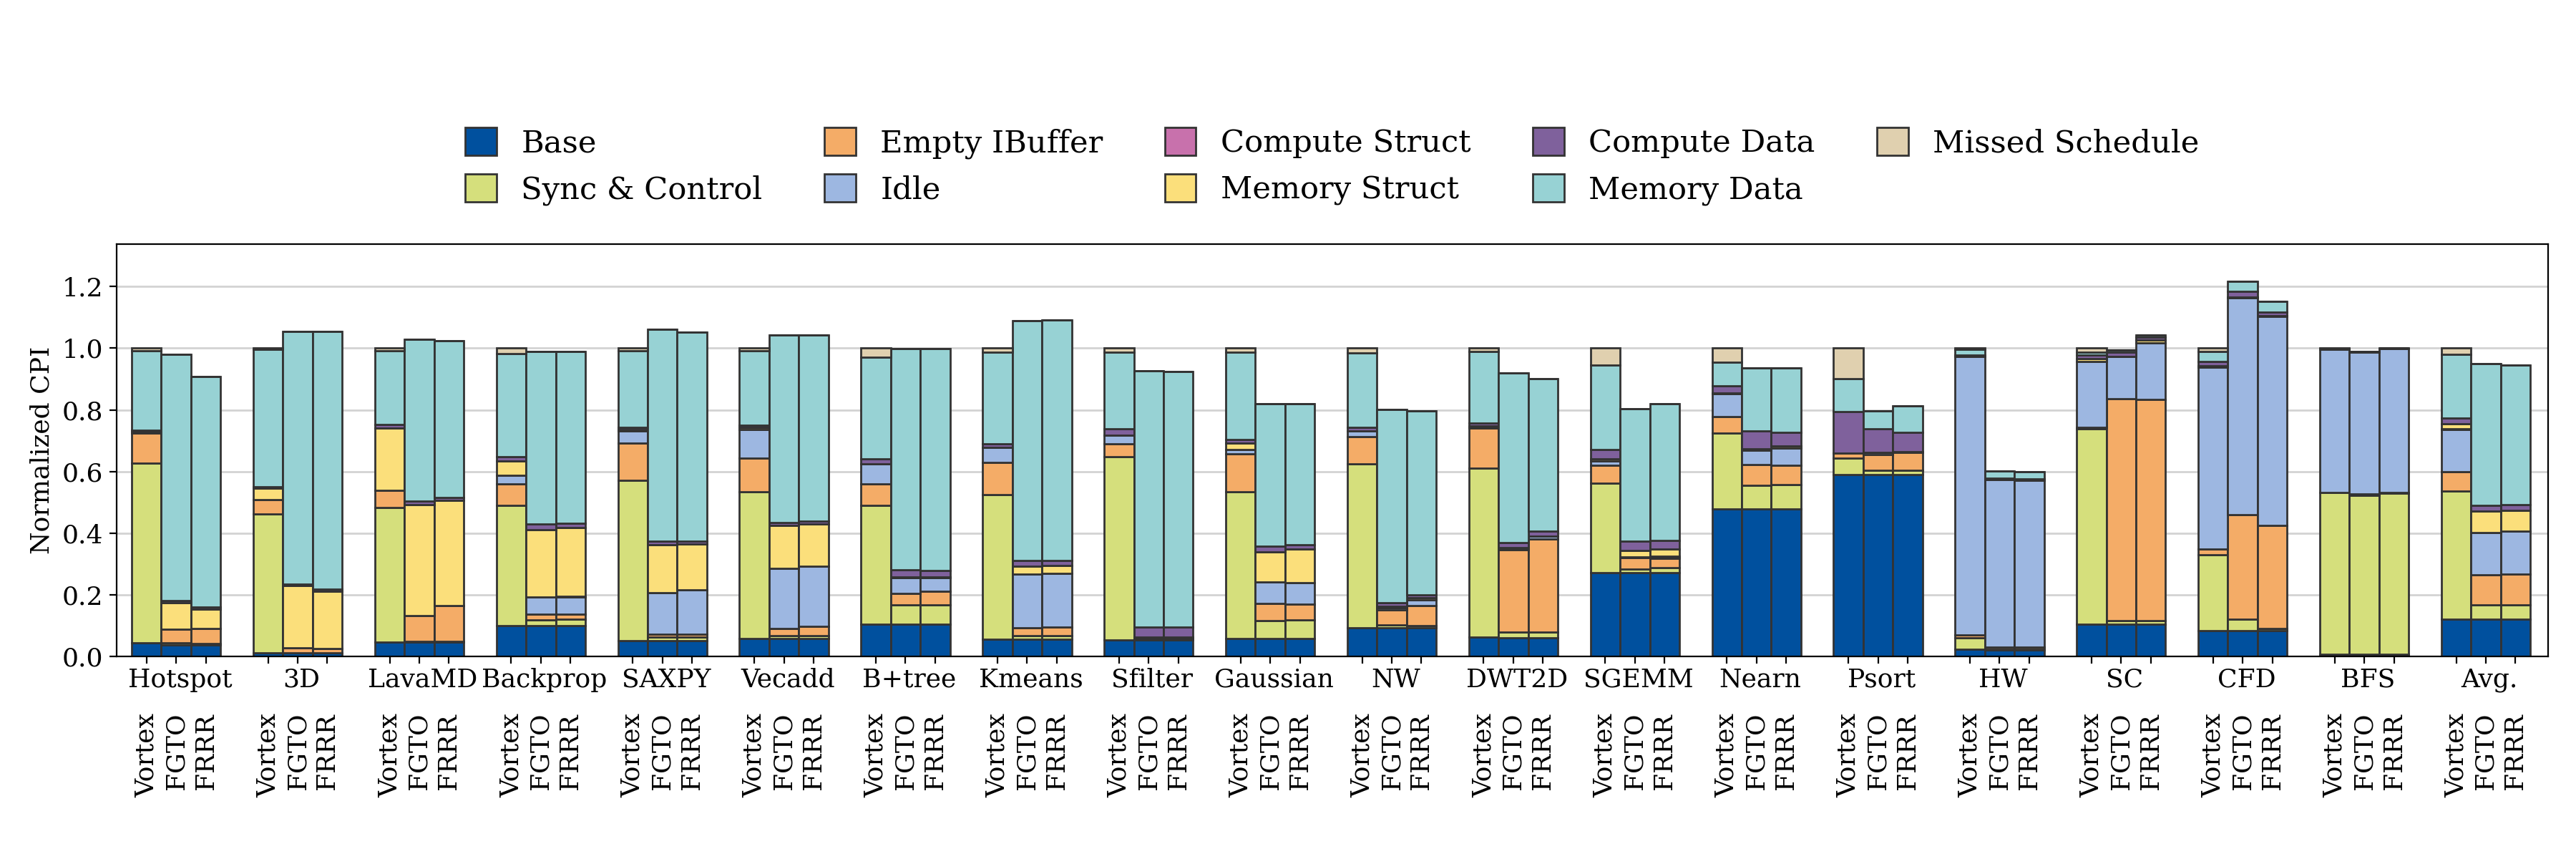
\includegraphics[width=1.3\textwidth]{figures/cpi_norm/L2.png}}
    \caption[Normalized \acrshort{cpi} stacks before and after the changes.]{Normalized \acrshort{cpi} stacks for the \Gls{vortex}, and the new \textit{GTO} and \textit{RRR} configurations}
    \label{fig:norm_cpi}
\end{figure}

Figure \ref{fig:norm_cpi} shows the \acrshort{cpi} stacks for all of the benchmarks, and the average \acrshort{cpi}, normalized to the baseline version. The changes to \Gls{vortex} have varying effects on the performance of each benchmark. In this context, performance is characterized by \acrshort{cpi}, where lower \acrshort{cpi} equates to higher performance. On average the \textit{FGTO} and \textit{FRRR}  configurations respectively have a $5.03\%$ and $5.48\%$ reduction in \acrshort{cpi} compared to \textit{\Gls{vortex}}. There are however large deviations from this average. The \textit{HW} benchmark has an almost a $40\%$ reduction in \acrshort{cpi} for both \textit{FGTO} and \textit{FRRR}, while \textit{CFD} see over $20\%$ increase in \acrshort{cpi} for the \textit{FGTO} configuration. Most of the benchmarks see a drastic shift in the causes of the stalls. This shift does however not necessarily reflect in an increase or decrease in \acrshort{cpi}. In the following sections, I will present subsets of the results shown in Figure \ref{fig:norm_cpi}, to explain the effects of the implemented changes.

\newpage
\section{Reduction of Control Stalls} \label{sec:result_control_stalls}

Figure~\ref{fig:norm_cpi_frontend} shows the normalized \acrshort{cpi} attributed to frontend stalls and base. It is clear that the frontend is the dominating cause for stalling in the baseline version. On average, 50\% of the \acrshort{cpi} is attributed to \textit{sync \& control} or \textit{empty ibuffer} stalls. \textit{Sync \& control} stalls are however most prevalent, representing over 40\% of the \acrshort{cpi}. \acrshort{nss}, and stall-prediction reduces the number of control stalls by removing unnecessary stalls. Because of this, warps are now only blocked after fetching instructions capable of changing the control flow or thread mask. The new icache-stage, enables \Gls{vortex} to perform multiple concurrent instruction fetches, which increases the fetch bandwidth. After implementing the new frontend, less than $5\%$ of the average \acrshort{cpi} is \textit{sync \& control} stalls, and the average \acrshort{cpi} attributed to the frontend is reduced by $71\%$. This shows that most instructions were unnecessarily blocked by the frontend. 

% 0.0002%
For \textit{sfilter}, \textit{FGTO} and \textit{FRRR} reduces the number of frontend stalls from $61\%$ to less than $0.01\%$ of the \textit{\Gls{vortex}} \acrshort{cpi}. This is because \textit{sfilter} does not have any branch instructions in its kernel, the warp scheduler can thus continue to fetch instructions without stalling. The few occurring frontend stalls are during the end of the benchmark. As the instructions are never blocked in the warp scheduler, the \acrshort{gto} warp scheduler would never switch which \acrshort{tb} it schedules from. However, \acrshort{bpr} informs the warp scheduler when the ibuffer is full, blocking the warp from being scheduled. \acrshort{bpr} is thus making the \acrshort{gto} warp scheduler switch if the backend is stalling, making it schedule more fairly. This becomes apparent as there are no idle stalls caused by \acrshortpl{tb} completing before others. This demonstrates how the new frontend is capable of removing all unnecessary control stalls.

While the new frontend has a large impact on most benchmarks, \textit{BFS} seems unable to utilize \acrshort{nss}. The number of \textit{sync \& control} stalls does not change between \textit{\Gls{vortex}}, \textit{FGTO} and \textit{FRRR}. A large proportion of \textit{BFS}' kernel are instructions pertaining to control flow and handling of divergence. Because of this, \textit{BFS} has a considerable number of required frontend stalls, which cannot be improved by \acrshort{nss}. Stall prediction ensures that these control stalls are not mispredicted. If the control-flow instructions were not stalled, it would waste many cycles having to flush the frontend. Stall-prediction is thus ensuring that the new frontend performs at least as well as the baseline in terms of control stalls. 

\begin{figure}
    \centering
    \makebox[\textwidth][c]{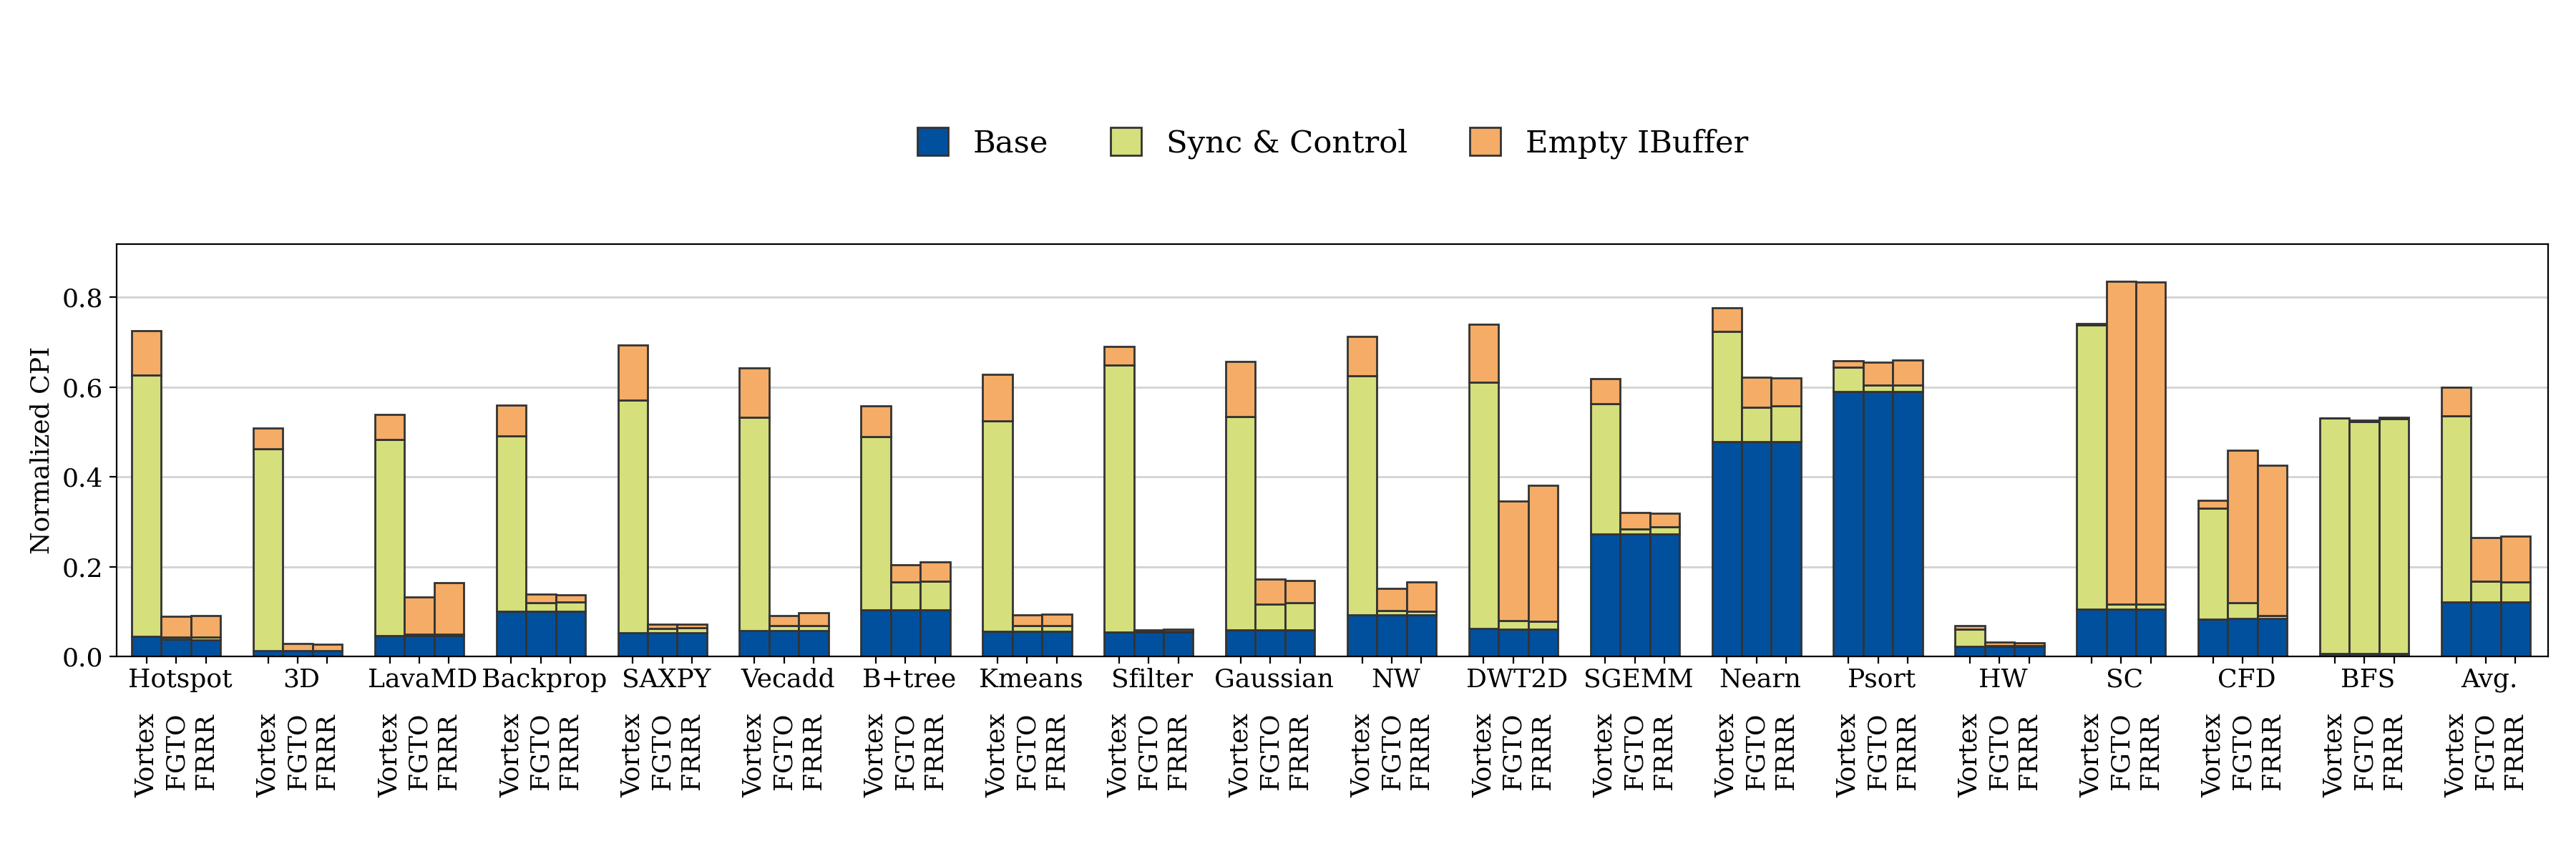
\includegraphics[width=1.3\textwidth]{figures/cpi_norm/cpi_frontend.png}}
    \caption[Normalized \acrshort{cpi} attributed to the frontend]{Normalized CPI attributed to the base cycles and stalls caused by the frontend.}
    \label{fig:norm_cpi_frontend}
\end{figure}

In the baseline configuration, all of the benchmarks have $5-10\%$ of the \acrshort{cpi} attributed to \textit{empty ibuffer}. These occur when a \acrshort{tb} has no warps available in the instruction buffer, and it is not currently blocked in the warp scheduler. Some of these stall cycles are caused by the latency between the warps being un-stalled, and then being fetched, decoded and sent to the ibuffer. For all the benchmarks, excluding \textit{lavaMD, DWT2D, SC} and \textit{CFD}, the number of \textit{empty-ibuffer} stalls are reduced. As the new frontend is able to cut down on the number of frontend stalls, the number of un-stalls is also reduced, which in turn reduces \textit{empty ibuffer} stalls.

Figure \ref{fig:norm_cpi} shows that \textit{SC} has almost no stalls related to the backend for any of the configurations. That is, when a warp arrives in the ibuffer, it is issued within a few cycles. For \textit{SC}, only the \textit{memset} kernel is executed, because of early-exit. The \textit{memset} kernel has almost no data dependencies. Thus the backend is almost never stalling, and the ibuffer is thus being emptied faster than it is filled. The \textit{memset} kernel has a short loop containing a memory write. The loop does require the frontend to stall, due to control flow. There are however no \textit{sync \& control} stalls shown for the \textit{FGTO} and \textit{FRRR} configurations, only \textit{empty ibuffer} stalls. This is because while the warp is stalled in the frontend, all previously fetched warps are issued, which hides the control stalls. When the control stall is released, all of the ibuffers are empty, causing \textit{empty ibuffer} stalls. Yet, there are more \textit{empty ibuffer} stalls when using the new frontend than \textit{sync \& control} stalls in the baseline version. This is likely because the icache-stage requires an additional cycle to reorder the icache responses. This results in a somewhat higher latency between a warp being fetched and it arriving in the ibuffer. A similar effect can be seen for other benchmarks such as \textit{srad} and \textit{CFD}. This problem can probably be solved by having a wider frontend, allowing for scheduling more than one instruction per cycle, or having enough warps per \acrshort{sm} to hide the frontend latency.

% memset inner loop
% 80000118: 33 05 c7 00                  	add	a0, a4, a2
% 8000011c: 23 00 b5 00                  	sb	a1, 0(a0)
% 80000120: 13 06 16 00                  	addi	a2, a2, 1
% 80000124: 33 35 f6 00                  	sltu	a0, a2, a5
% 80000128: 6b 00 15 00                  	vx_pred	a0            ; Control stall
% 8000012c: e3 66 f6 fe                  	bltu	a2, a5, -20   ; Control stall

\section{Utilization of Functional Units}

\begin{figure}
    \centering
    \makebox[\textwidth][c]{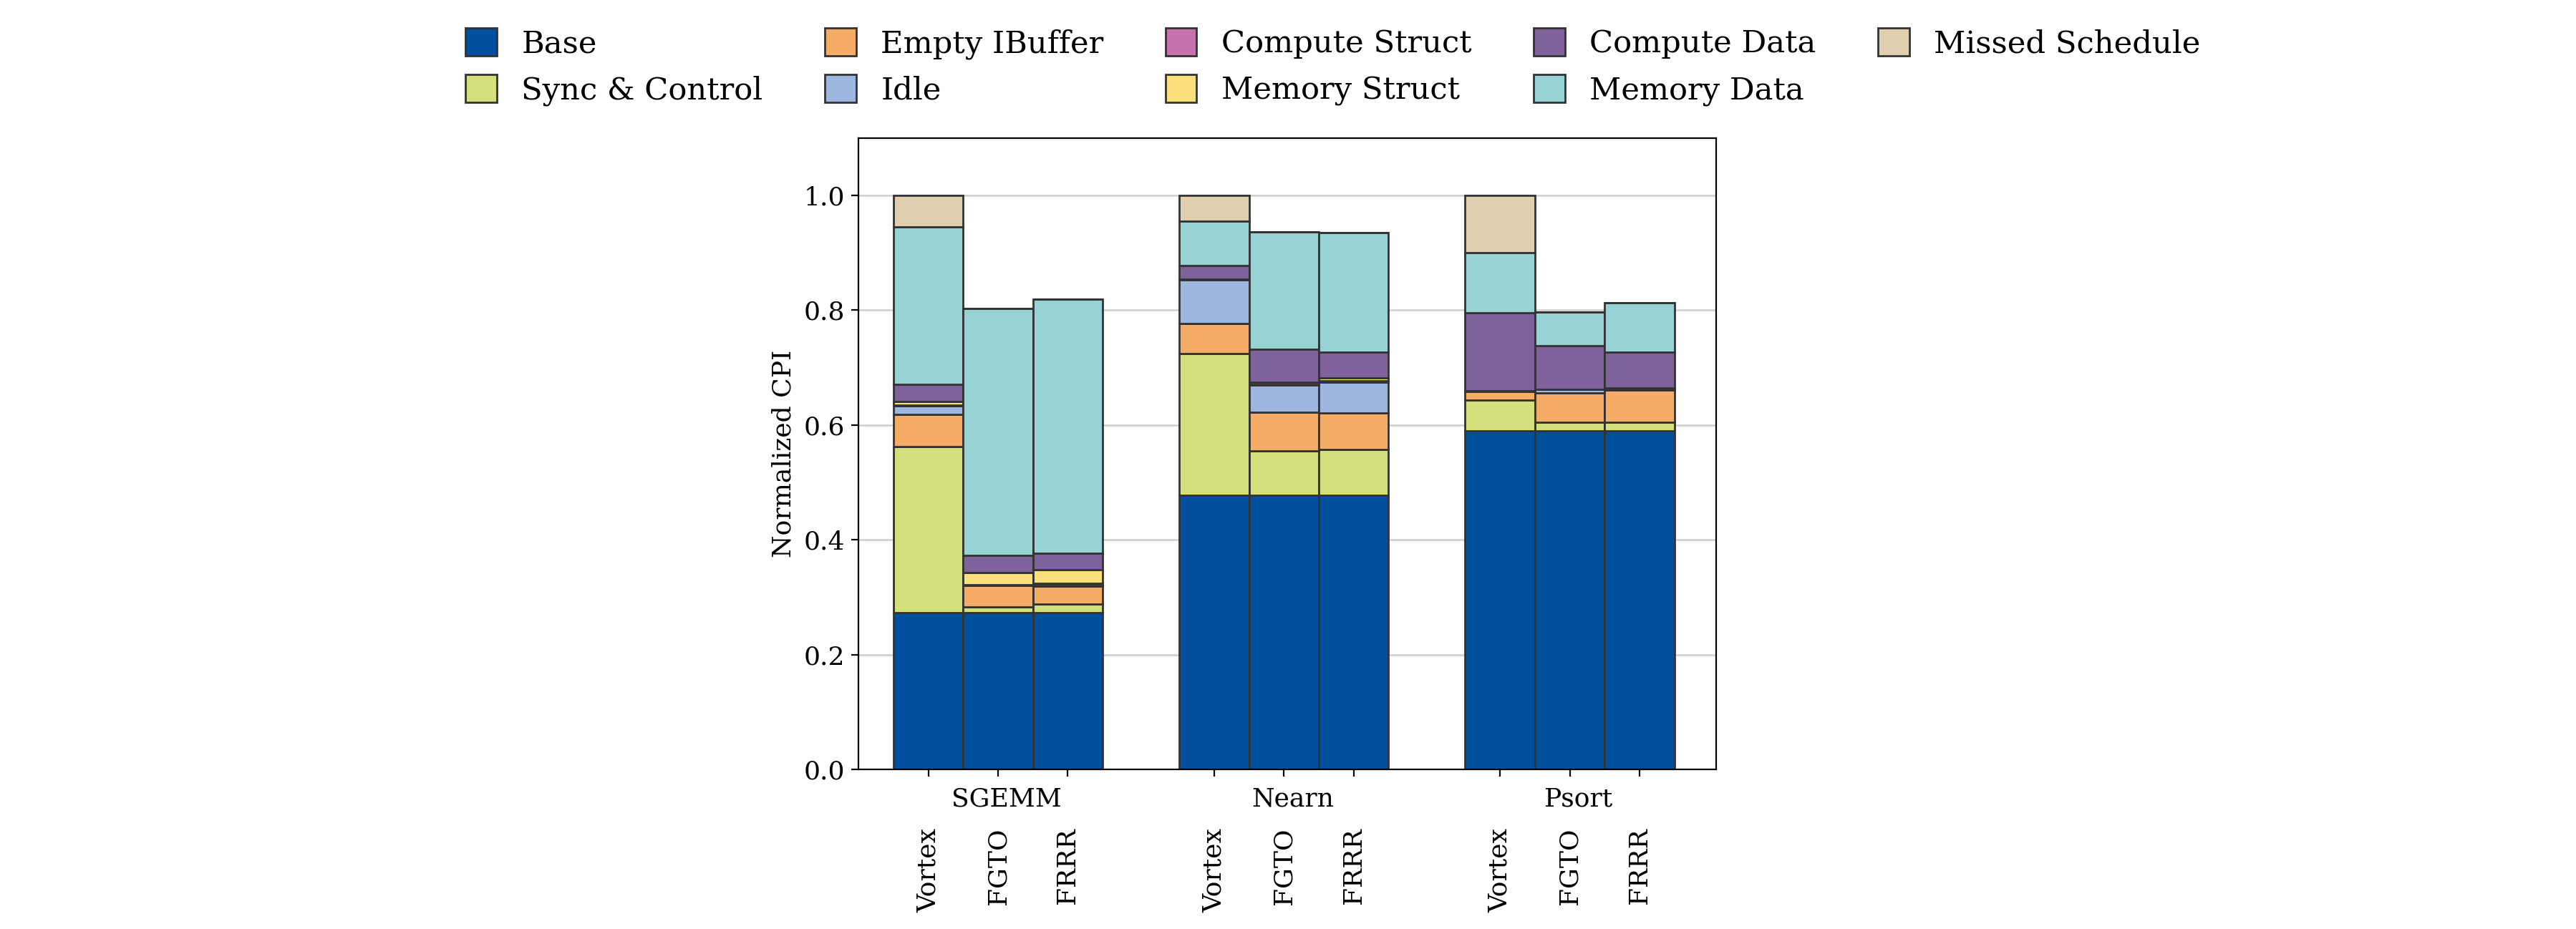
\includegraphics[width=1.3\textwidth]{figures/cpi_norm/missed_schedule_wide.png}}
    \caption[Normalized \acrshort{cpi} for benchmarks with most missed schedule opportunities.]{Normalized \acrshort{cpi} for benchmarks with most \textit{missed schedule} stalls.}
    \label{fig:cpi_missed_schedule}
\end{figure}

Figure \ref{fig:cpi_missed_schedule} shows the \acrshort{cpi} stacks of the benchmarks with the largest proportion of \textit{missed schedule} stalls. For \textit{psort}, the number of stalls is nearly halved for both \textit{FGTO} and \textit{FRRR}, resulting in a $20\%$ decrease in \acrshort{cpi} compared to the \textit{\Gls{vortex}} configuration. \textit{Psort} has a low number of frontend stalls, which does not change after implementing the new frontend, as nearly all \textit{sync \& control} stalls are replaced by \textit{empty ibuffer} stalls. \textit{Psort} is thus seeing limited improvements from the frontend changes. The implementation of ready scheduling in \textit{FGTO} and \textit{FRRR} is able to remove all the \textit{missed schedule} stalls. In the \textit{\Gls{vortex}} configuration, \textit{missed schedule} stalls contribute to about $10\%$ of the \acrshort{cpi}, while for \textit{FGTO} the \acrshort{cpi} is decreased by the double ($20\%$). This is because other than frontend and \textit{missed schedule}, \textit{psort} is stalled by compute data dependencies. These stalls can be hidden by the increased number of issued instructions, as they have low latency.

The \textit{sgemm} and \textit{nearn} benchmarks also have a significant number of \textit{missed schedule} stalls. In addition to the improvements obtained by ready scheduling, these benchmarks see a great reduction in frontend stalls. The increased throughput of the frontend makes more warps available in the issue stage, increasing the effect of ready scheduling. Because of the significant decrease in frontend stalls, \textit{sgemm} is also able to obtain a $20\%$ reduction in \acrshort{cpi}. This is similar to \textit{psort}, but with a smaller proportion of \textit{missed schedule} stalls in the \textit{\Gls{vortex}} configuration. The \acrshort{cpi} of \textit{nearn} is not reduced to the same degree as \textit{sgemm} and \textit{psort}. This is likely caused by a combination of multiple factors. The number of frontend stalls is only halved, thus revealing fewer additional warps in the ibuffer than \textit{sgemm}. \textit{Nearn} also have less \textit{missed schedule} stalls than \textit{psort} and more long-latency \textit{memory data} stalls than \textit{psort}. Because of this, there are fewer stalls which can be hidden by ready scheduling.

\section{Memory Stalls} \label{sec:results_memory}

\begin{figure}
    \centering
    \makebox[\textwidth][c]{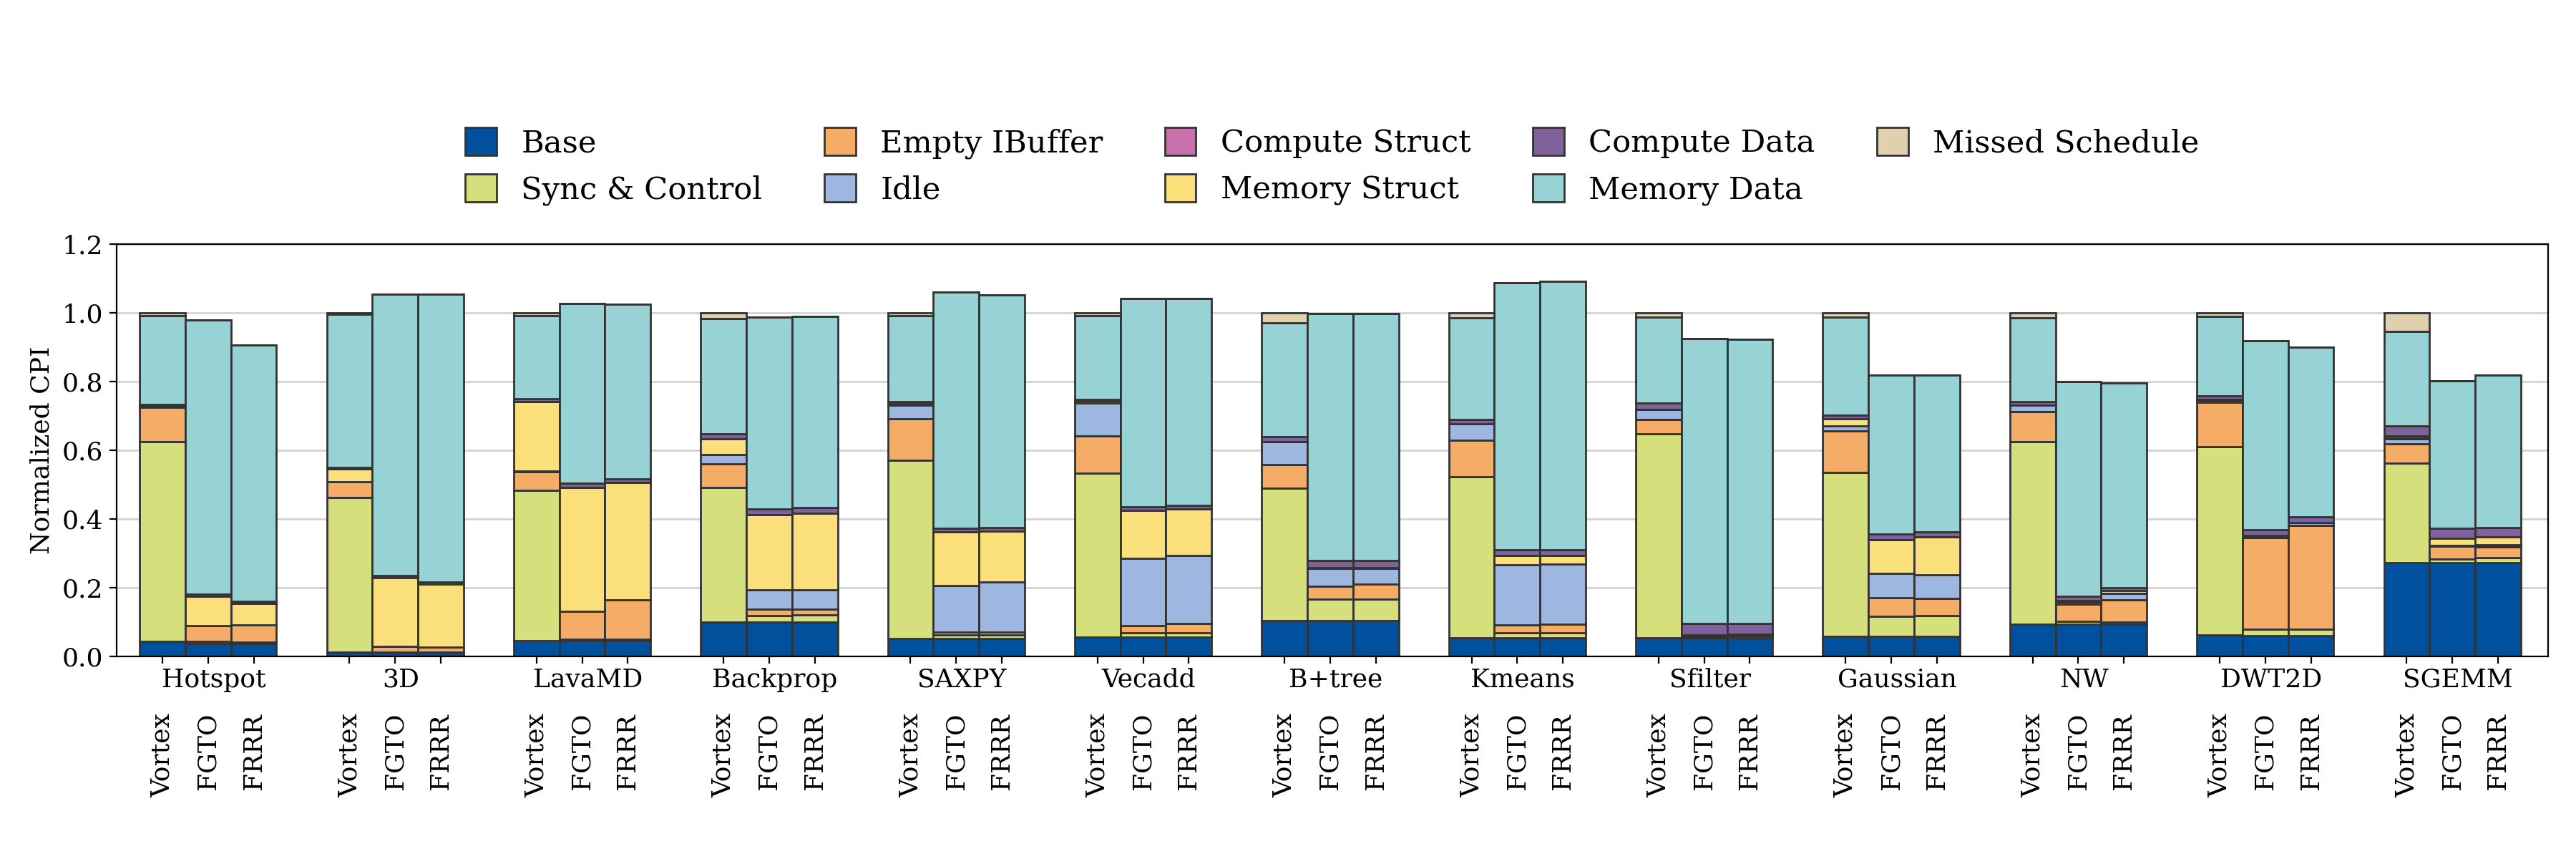
\includegraphics[width=1.3\textwidth]{figures/cpi_norm/exposed_memory.png}}
    \caption[Normalized \acrshort{cpi} for benchmarks where memory stalls are revealed]{Normalized \acrshort{cpi} for benchmarks where memory stalls are revealed using \textit{FGTO} and \textit{FRRR}}
    \label{fig:exposed_memory}
\end{figure}

\begin{figure}
    \centering
    \makebox[\textwidth][c]{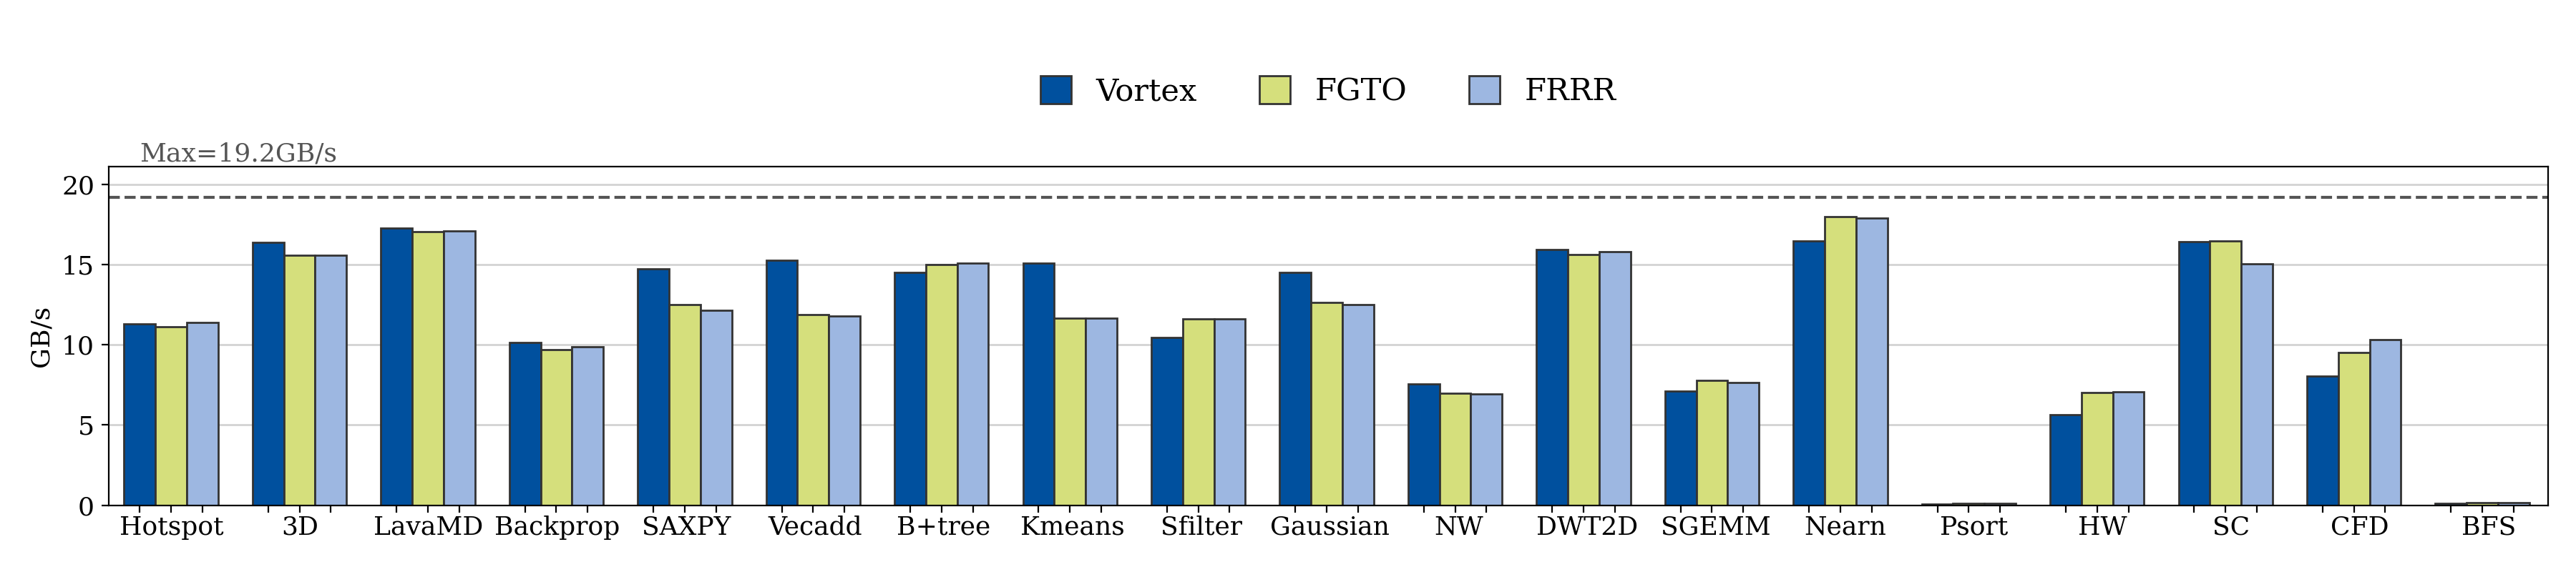
\includegraphics[width=1.3\textwidth]{figures/bandwidth/L2.png}}
    \caption[Average bandwidth usage between the L2 cache and main memory.]{Average bandwidth usage between the L2 cache and DDR4 memory}
    \label{fig:bandwidth_usage_l2}
\end{figure}

\begin{figure}
    \centering
    \begin{subfigure}{\textwidth}
         \centering
         \makebox[\textwidth][c]{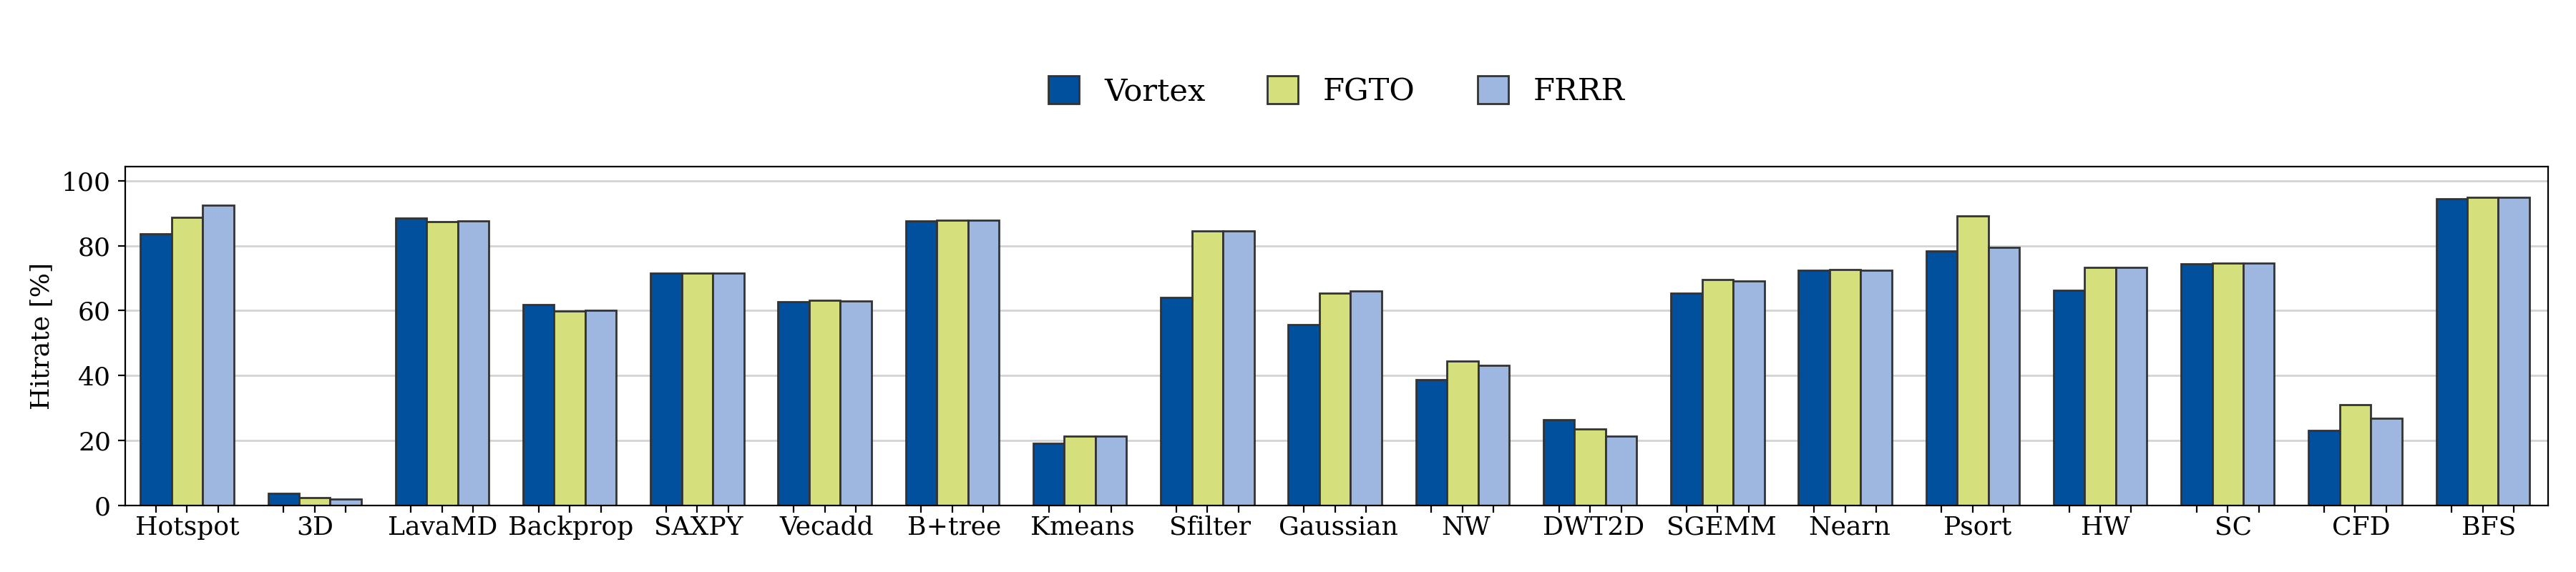
\includegraphics[width=1.3\textwidth]{figures/L1_dcache_hitrate/L2.png}}
         \caption{L1 dcache hitrate}
         \label{fig:l1_dcache_hitrate}
     \end{subfigure}
     \hfill
         \begin{subfigure}{\textwidth}
         \centering
         \makebox[\textwidth][c]{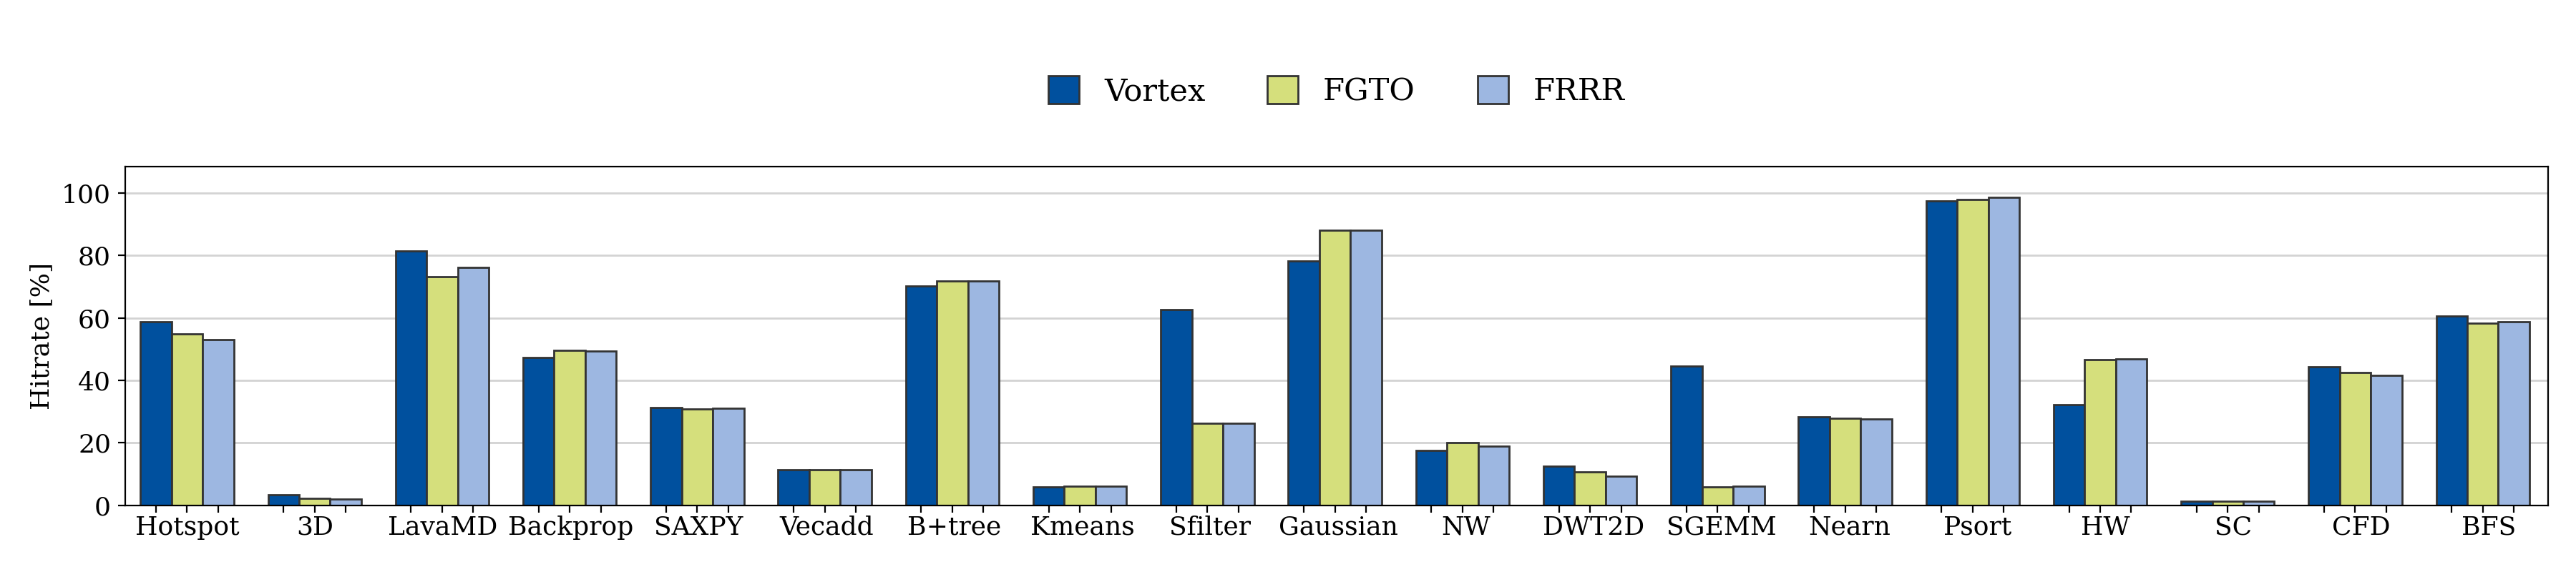
\includegraphics[width=1.3\textwidth]{figures/L2_dcache_hitrate/L2.png}}
         \caption{L2 dcache hitrate}
         \label{fig:l2_dcache_hitrate}
    \end{subfigure}
    \caption{Average dcache hitrate}
    \label{fig:dcache_hitrate}
\end{figure}

Figure \ref{fig:exposed_memory} shows the normalized \acrshort{cpi} stacks for the benchmarks where \textit{FGTO} and \textit{FRRR} reveal memory stalls. For all of these benchmarks, a significant number of \textit{memory data} stalls are revealed. Additionally for \textit{hotspot, 3D, lavaMD, saxpy, vecadd} and \textit{gaussian}, \textit{memory structural} stalls are also uncovered. As there is an increase in \textit{memory structural} stalls it would be rational to assume an increase in memory bandwidth usage. However, the memory bandwidth usage illustrated in Figure \ref{fig:bandwidth_usage_l2}, shows the opposite. For the benchmarks where the changes expose \textit{memory structural} stalls, the bandwidth is either decreased or unchanged. Figure \ref{fig:l1_dcache_hitrate} and \ref{fig:l2_dcache_hitrate} show that the dcache hitrates are similar for \textit{\Gls{vortex}}, \textit{FGTO} and \textit{FRRR}. This indicates that there are other causes for the \textit{memory structural} stalls.

\textit{Backprop} and \textit{lavaMD} both have a large number of \textit{memory structural} stalls, but very different bandwidth utilization. \textit{LavaMD} use $17GB/s$ of memory bandwidth on average while \textit{backprop} use $10GB/s$, which is only about half of the available bandwidth. For \textit{lavaMD}, the available bandwidth is likely the main cause of \textit{memory structural} stalls, as its average usage is close to the available bandwidth. This is not the case for \textit{backprop}. Unlike \textit{lavaMD}, \textit{backprop} uses a lot of memory barriers. When a memory barrier is issued to the \acrshort{lsu}, all in-flight memory instructions have to complete before the \acrshort{lsu} will be ready. \textit{Memory structural} stalls are therefore occurring while these barriers are resolving. Because of this, the average memory bandwidth usage can be low while still producing \textit{memory structural} stalls. This is also why \textit{hotspot} has an increase in \textit{memory structural} stalls. It is however a smaller increase, as it is dependant on the latency of the requests and the frequency of the barrier instructions.

For all of the benchmarks in Figure~\ref{fig:exposed_memory}, a large number of \textit{memory data} stalls are revealed when \textit{FGTO} and \textit{FRRR} reduce frontend stalls. Because warps are waiting for the results of memory requests, these stalls are caused by memory latency. It is most likely that these memory requests are already in-flight, and thus the increased frontend throughput just exposes the stall sooner. As there is such a large proportion of \textit{memory data} stalls, it is clear that \Gls{vortex} is incapable of hiding them. There is simply not enough work to do while waiting for the memory requests. The average latency for each benchmark is shown on a logarithmic scale in Figure \ref{fig:avg_mem_latency}. It is a clear trend that \textit{FGTO} and \textit{FRRR} is increasing the memory latency. This is likely because the memory requests are being queued in the memory system. It is possible that \textit{FRRR} and \textit{FGTO} make the memory requests within a shorter time span than \textit{\Gls{vortex}}, due to the frontend throughput. This would generate uneven memory bandwidth usage, and result in queuing. This would explain why the latency is increased, while the average bandwidth does not. Section~\ref{sec:results_warp_scheduling} will discuss further why \textit{FGTO} does not perform better than \textit{FRRR} in this situation.

\begin{figure}
    \centering
    \makebox[\textwidth][c]{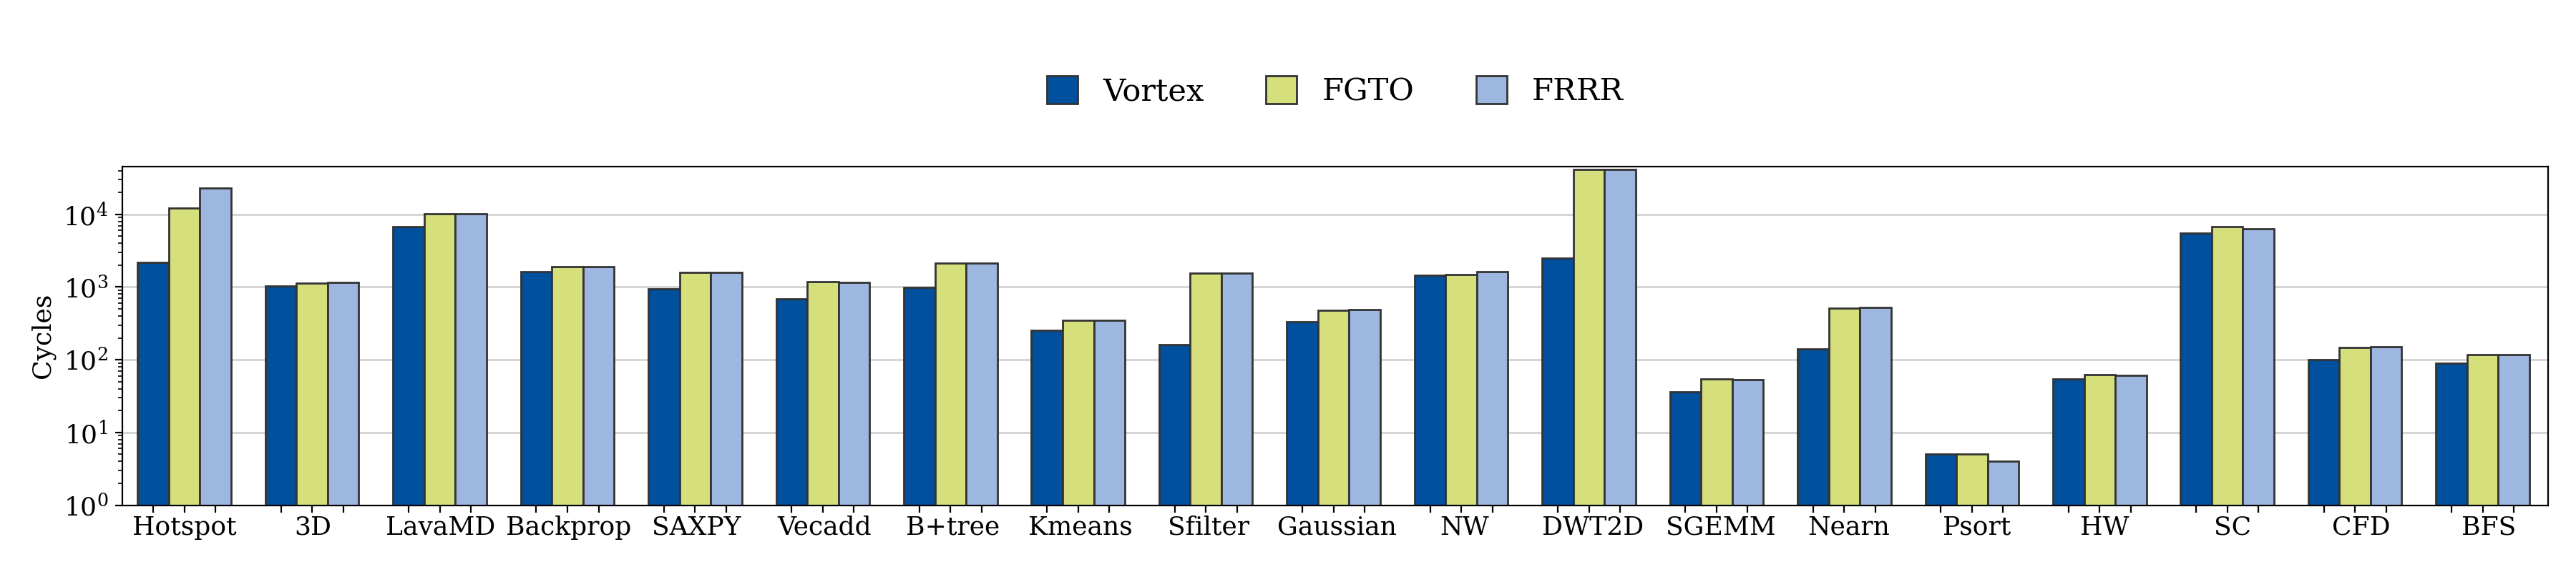
\includegraphics[width=1.3\textwidth]{figures/latency/L2.png}}
    \caption{Average memory latency on logarithmic scale}
    \label{fig:avg_mem_latency}
\end{figure}

Figure~\ref{fig:dcache_hitrate} shows the L1 and L2 dcache hit rates for all the benchmarks. For most of the benchmarks, the configuration does not affect the L1 cache hit rate. However, \textit{hotspot, sfilter, gaussian} and \textit{NW} see a significant increase in L1 hit rate for \textit{FGTO} and \textit{FRRR} compared to \textit{\Gls{vortex}}. A potential cause of this increase is that \textit{\Gls{vortex}}' find-first warp scheduler is causing some warps to run ahead of others, making them evict cache lines of memory shared between the \acrshortpl{tb}. This is not happening when using \acrshort{gto} or \acrshort{lrr} warp scheduling as they schedule the warps more fairly.

\begin{figure}
    \centering
    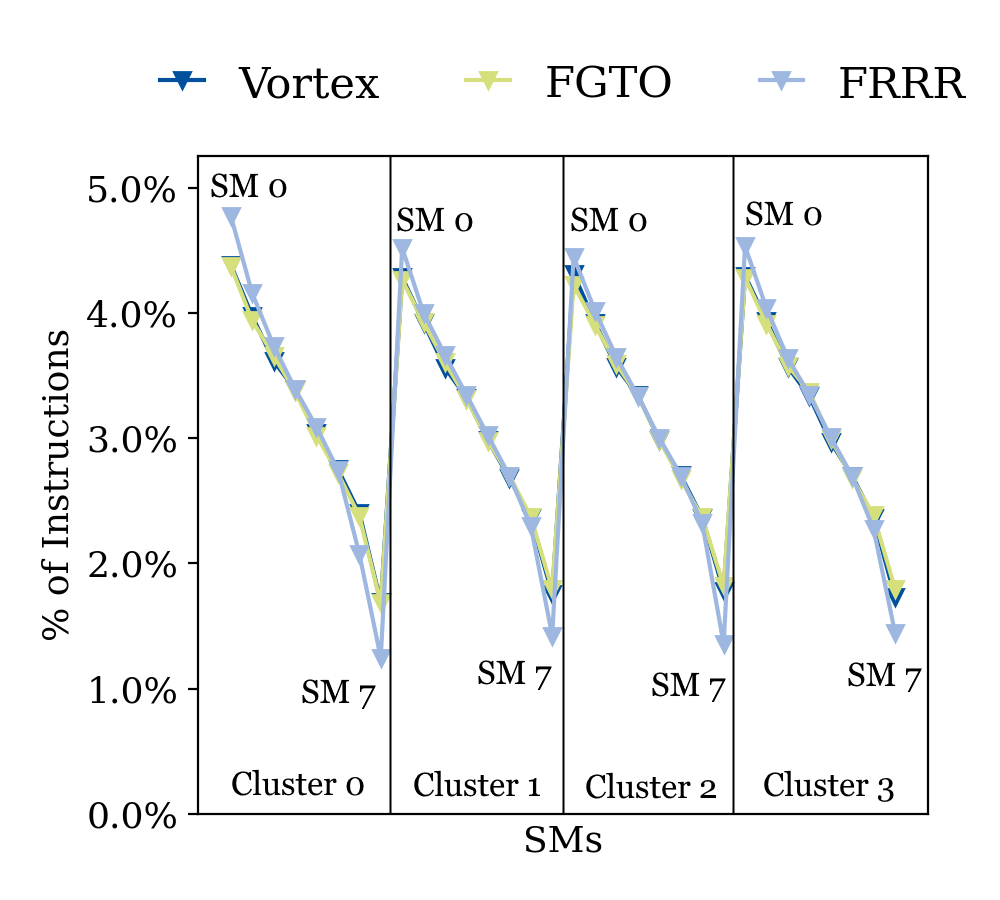
\includegraphics[width=0.8\textwidth]{figures/instruction_distribution/hotspot3D_unsorted_numbered.png}
    \caption[Distribution of executed instructions in clusters for Hotspot3D]{Distribution of executed instructions per \acrshort{sm} and cluster for Hotspot3D (3D)}
    \label{fig:instruction_distribution_unsorted_3D}
\end{figure}

Figure \ref{fig:instruction_distribution_unsorted_3D} shows the distribution of executed instructions by each of \Gls{vortex}' \acrshortpl{sm} for the \textit{3D} benchmark. It is clear that within each cluster, \textit{\acrshort{sm}0} is executing close to $5\times$ more instructions than \textit{\acrshort{sm}7}. For each increasing index within the cluster, the \acrshortpl{sm} are executing fewer instructions. As there are no idle cycles for \textit{3D}, this cannot be because less work is being allocated to the \acrshortpl{sm}. If the benchmark would have finished instead of exiting early, there would probably be idle cycles, as the \acrshortpl{sm} with lower indices would finish before the higher indexed \acrshortpl{sm}. The difference in the number of executed instructions is likely caused by the \acrshort{noc} distributing the available bandwidth unfairly. A similar effect can be observed for \textit{lavaMD} in figure \ref{fig:instr_dist_lavaMD}, as both \textit{lavaMD} and \textit{3D} exit early and have bandwidth utilization close to the available memory bandwidth.

\textit{SAXPY, vecadd, kmeans} and \textit{gaussian}, see a significant decrease in bandwidth utilization. This decrease is mainly caused by an increase in idle cycles. As some of the cores idle, they stop sending memory requests, lowering the average bandwidth utilization. Section \ref{sec:workload_dist} will explain further why these benchmarks idle.

\newpage
\section{Workload Distribution} \label{sec:workload_dist}

\begin{figure}
     \centering
     \makebox[\linewidth][c]{
     \begin{subfigure}[t]{0.3\textwidth}
         \centering
         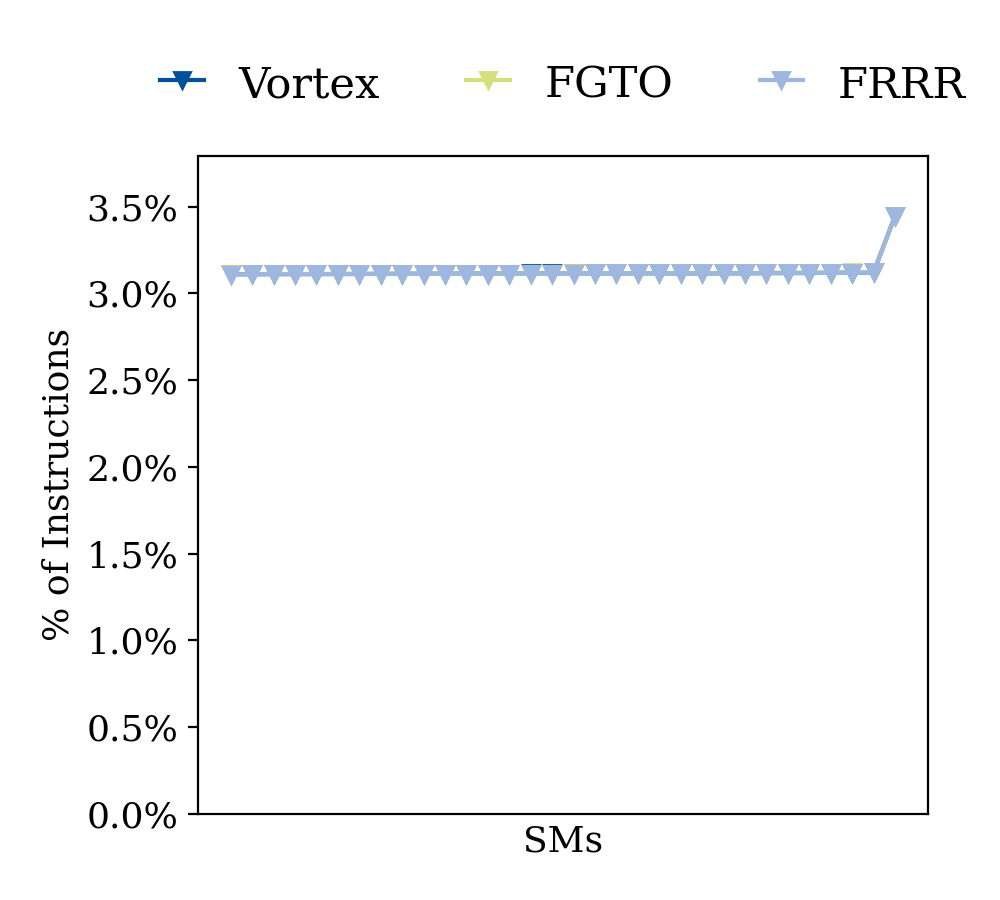
\includegraphics[width=\textwidth]{figures/instruction_distribution/b+tree_L2.png}
         \caption{B+Tree}
         \label{fig:instr_dist_btree}
     \end{subfigure}
     \hfill
         \begin{subfigure}[t]{0.3\textwidth}
         \centering
         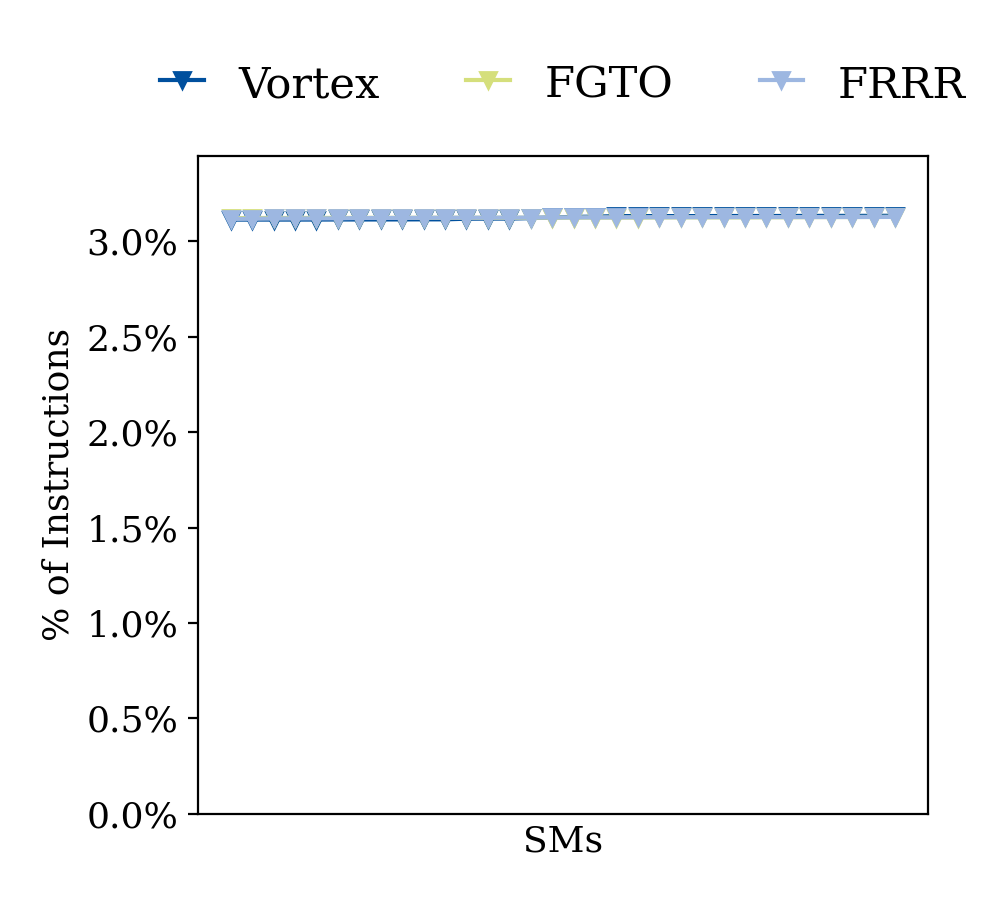
\includegraphics[width=\textwidth]{figures/instruction_distribution/backprop_L2.png}
         \caption{Backprop}
         \label{fig:instr_dist_backprop}
     \end{subfigure}
     \hfill
          \begin{subfigure}[t]{0.3\textwidth}
         \centering
         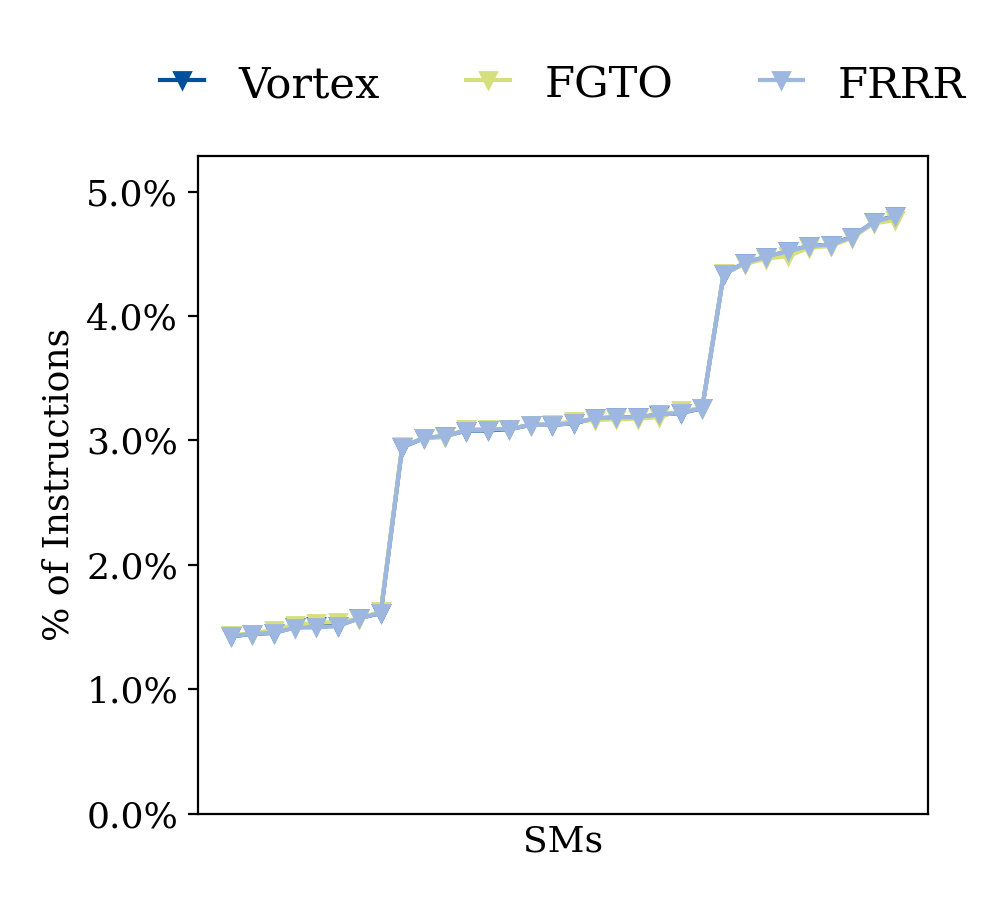
\includegraphics[width=\textwidth]{figures/instruction_distribution/bfs_L2.png}
         \caption{BFS}
         \label{fig:instr_dist_bfs}
     \end{subfigure}
     \hfill
          \begin{subfigure}[t]{0.3\textwidth}
         \centering
         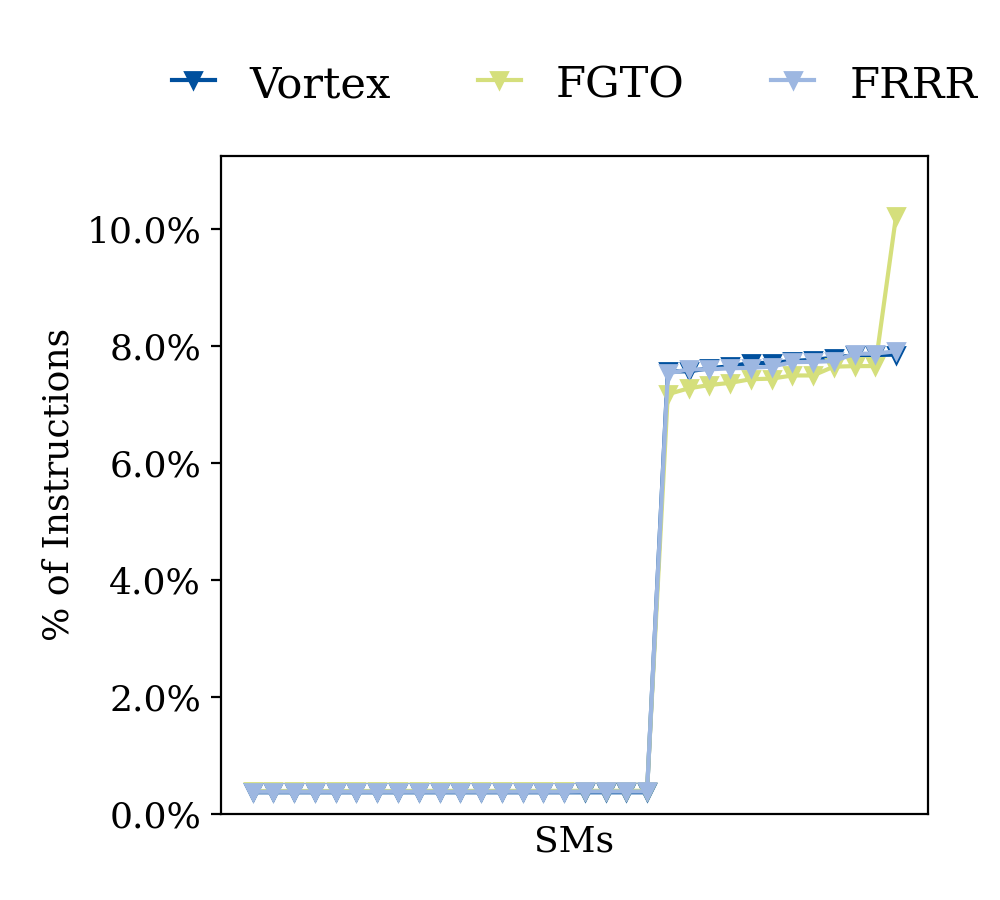
\includegraphics[width=\textwidth]{figures/instruction_distribution/cfd_L2.png}
         \caption{CFD}
         \label{fig:instr_dist_cfd}
     \end{subfigure}
     \hfill
     }

     \makebox[\linewidth][c]{
          \begin{subfigure}[t]{0.3\textwidth}
         \centering
         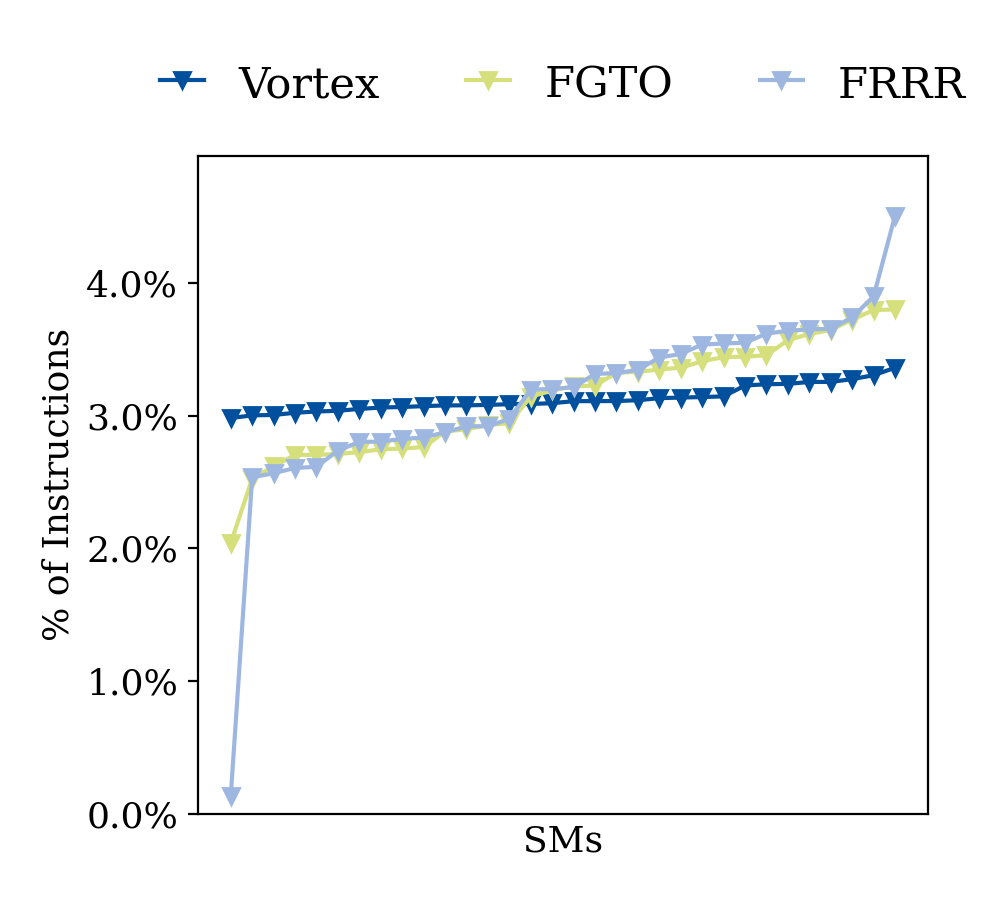
\includegraphics[width=\textwidth]{figures/instruction_distribution/dwt2d_L2.png}
         \caption{DWT2D}
         \label{fig:instr_dist_dwt2d}
     \end{subfigure}
     \hfill
          \begin{subfigure}[t]{0.3\textwidth}
         \centering
         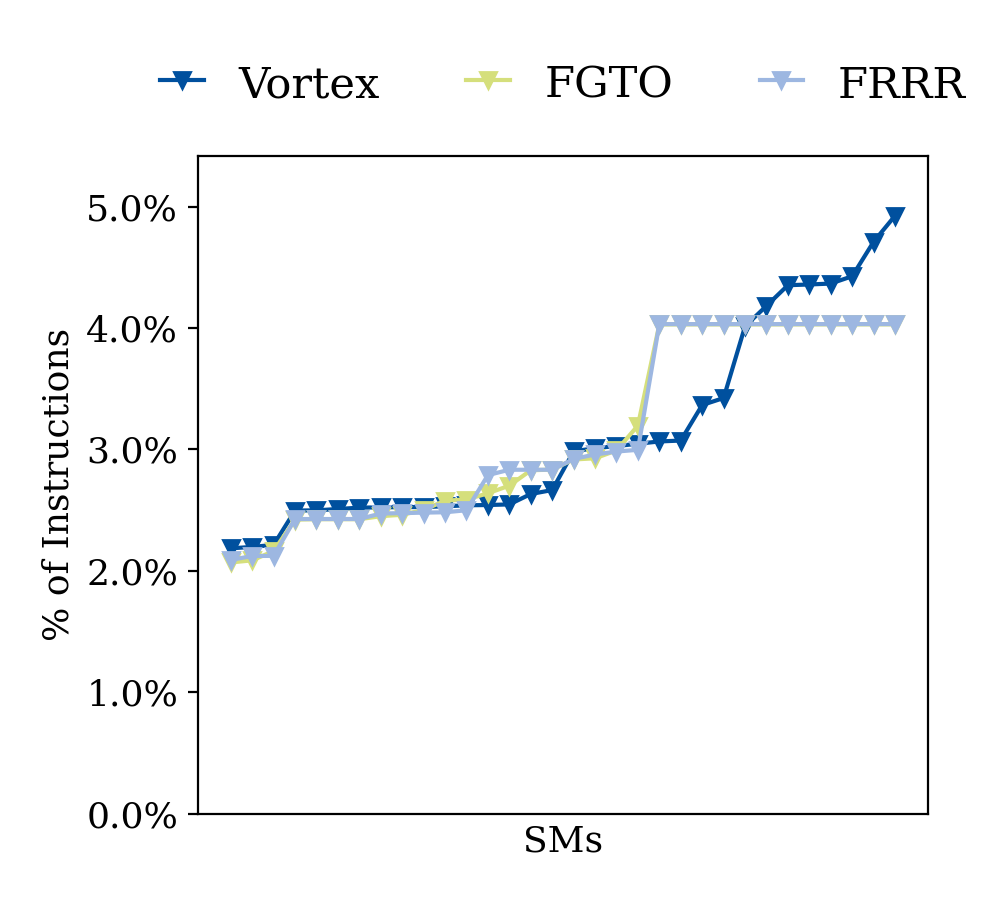
\includegraphics[width=\textwidth]{figures/instruction_distribution/gaussian_L2.png}
         \caption{Gaussian}
         \label{fig:instr_dist_gaussian}
     \end{subfigure}
     \hfill
          \begin{subfigure}[t]{0.3\textwidth}
         \centering
         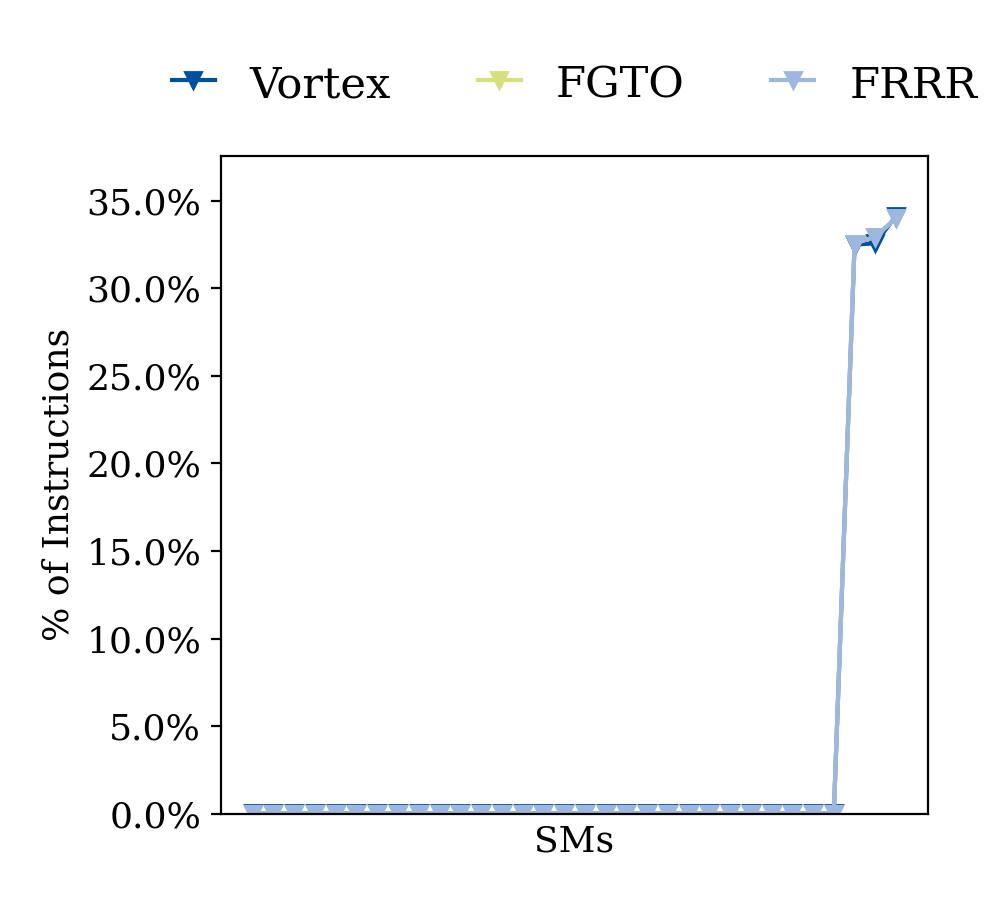
\includegraphics[width=\textwidth]{figures/instruction_distribution/heartwall_L2.png}
         \caption{HW}
         \label{fig:instr_dist_hw}
     \end{subfigure}
     \hfill
          \begin{subfigure}[t]{0.3\textwidth}
         \centering
         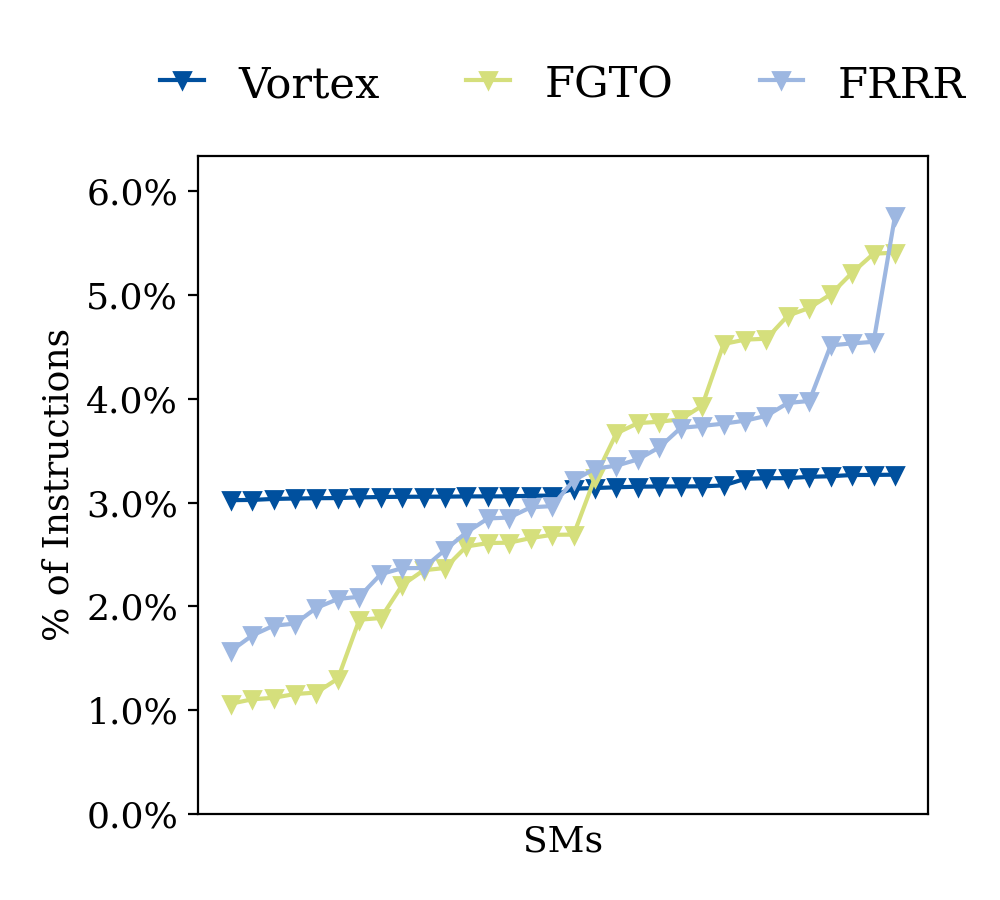
\includegraphics[width=\textwidth]{figures/instruction_distribution/hotspot_L2.png}
         \caption{Hotspot}
         \label{fig:instr_dist_hotspot}
     \end{subfigure}
     }
     
     \makebox[\linewidth][c]{
     \hfill
          \begin{subfigure}[t]{0.3\textwidth}
         \centering
         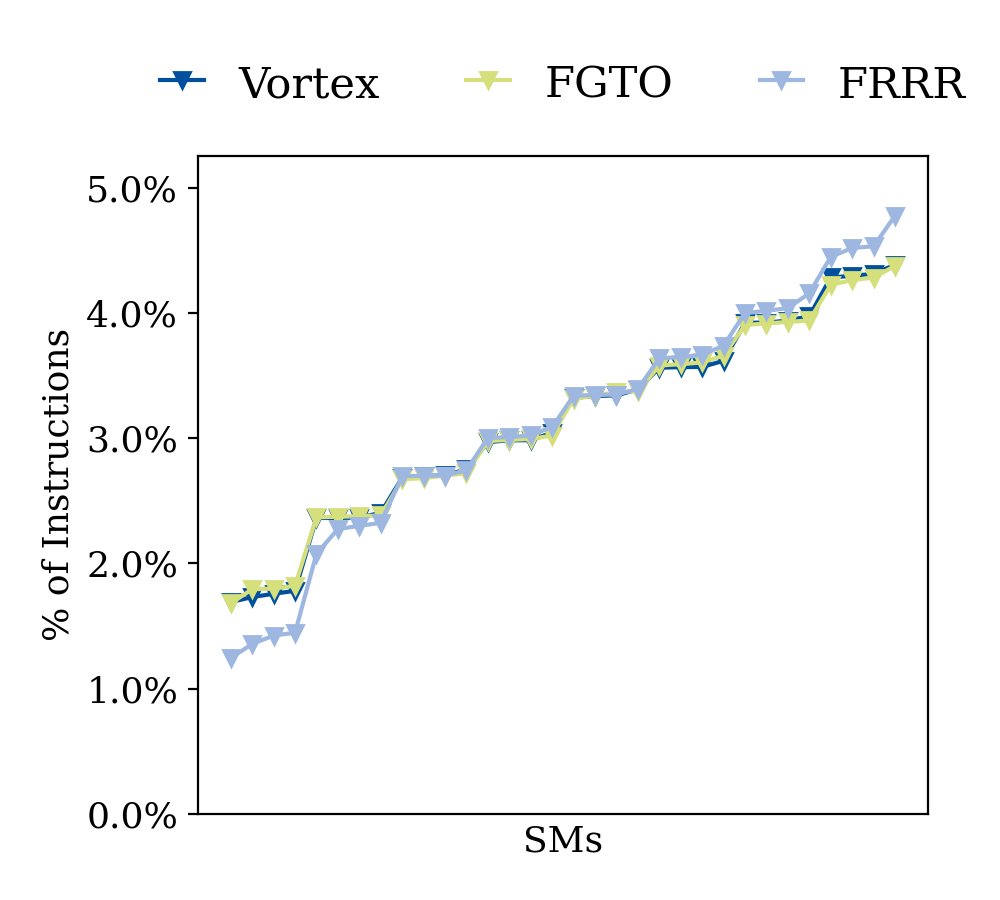
\includegraphics[width=\textwidth]{figures/instruction_distribution/hotspot3D_L2.png}
         \caption{3D}
         \label{fig:instr_dist_3d}
     \end{subfigure}
          \hfill
          \begin{subfigure}[t]{0.3\textwidth}
         \centering
         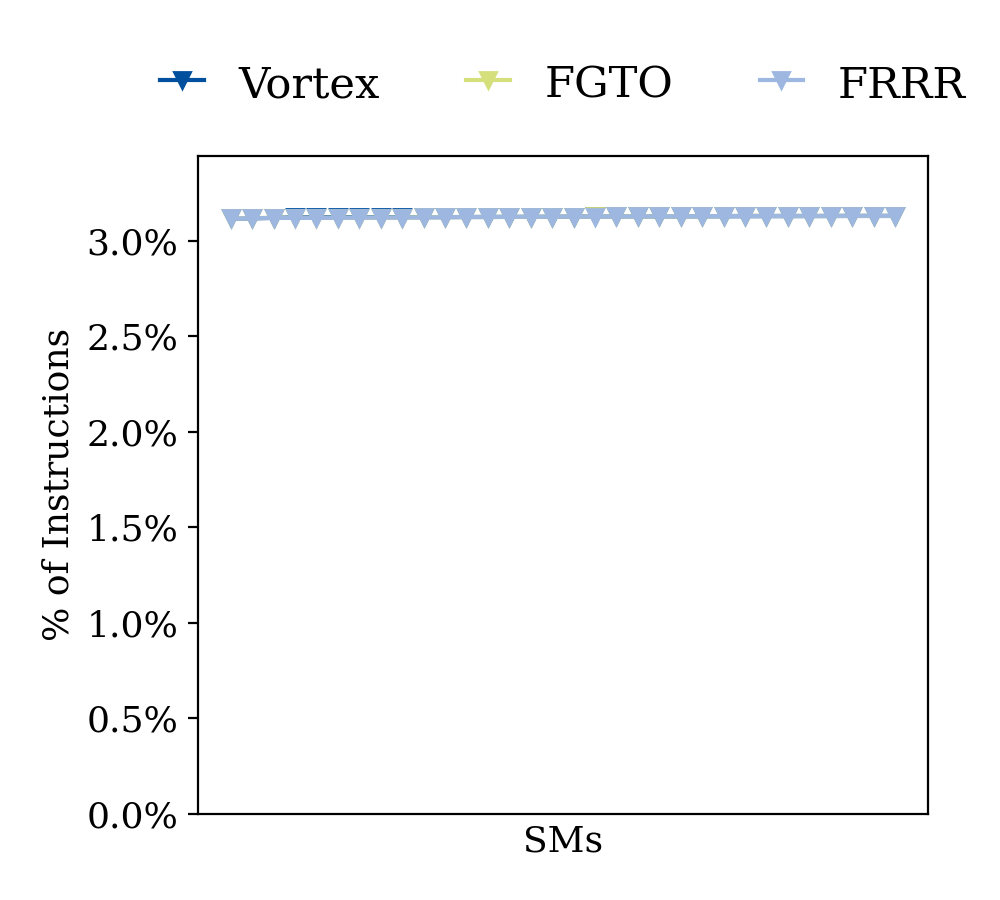
\includegraphics[width=\textwidth]{figures/instruction_distribution/kmeans_L2.png}
         \caption{Kmeans}
         \label{fig:instr_dist_kmeans}
     \end{subfigure}
          \hfill
          \begin{subfigure}[t]{0.3\textwidth}
         \centering
         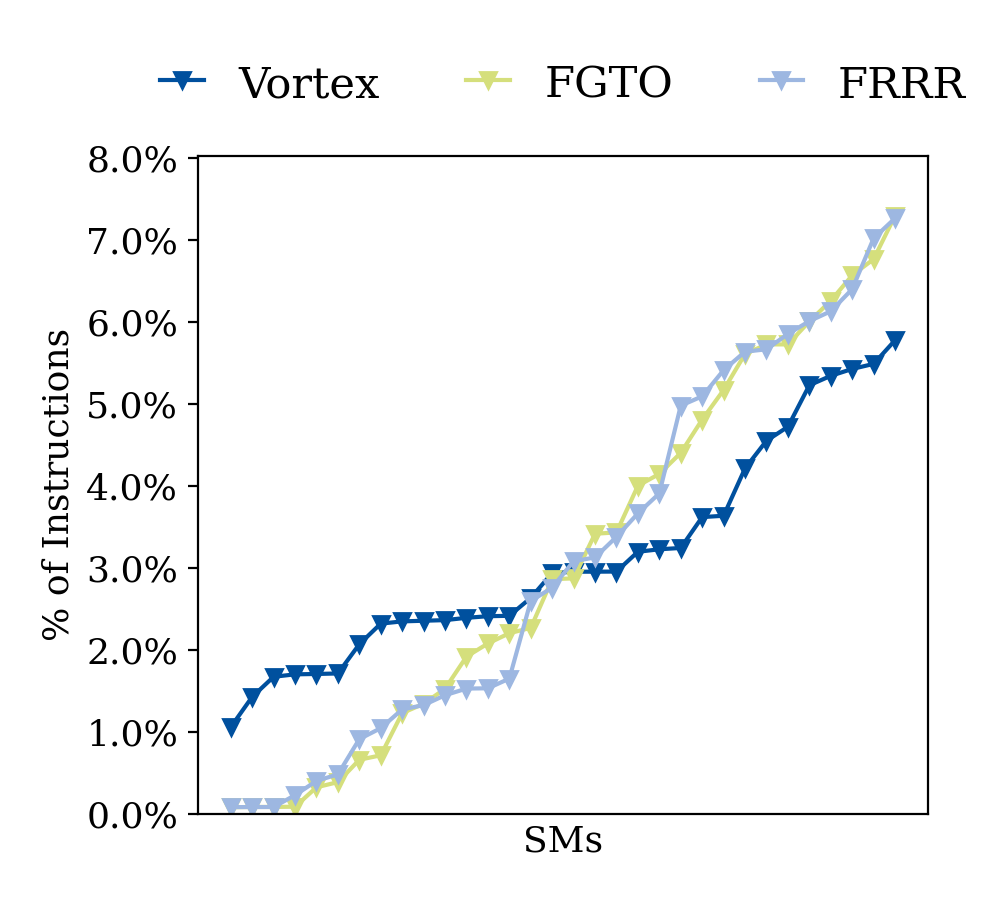
\includegraphics[width=\textwidth]{figures/instruction_distribution/lavaMD_L2.png}
         \caption{LavaMD}
         \label{fig:instr_dist_lavaMD}
     \end{subfigure}
          \hfill
          \begin{subfigure}[t]{0.3\textwidth}
         \centering
         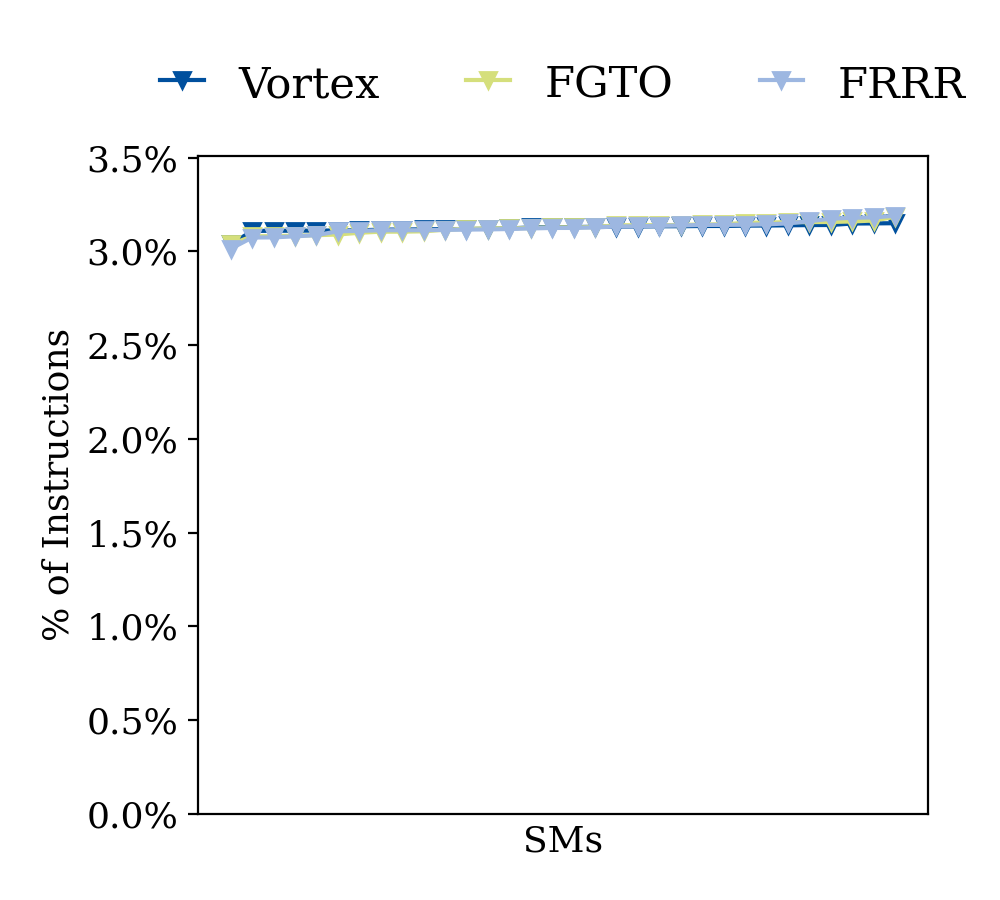
\includegraphics[width=\textwidth]{figures/instruction_distribution/nearn_L2.png}
         \caption{Nearn}
         \label{fig:instr_dist_nearn}
     \end{subfigure}
     }
     
    \makebox[\linewidth][c]{
     \hfill
          \begin{subfigure}[t]{0.3\textwidth}
         \centering
         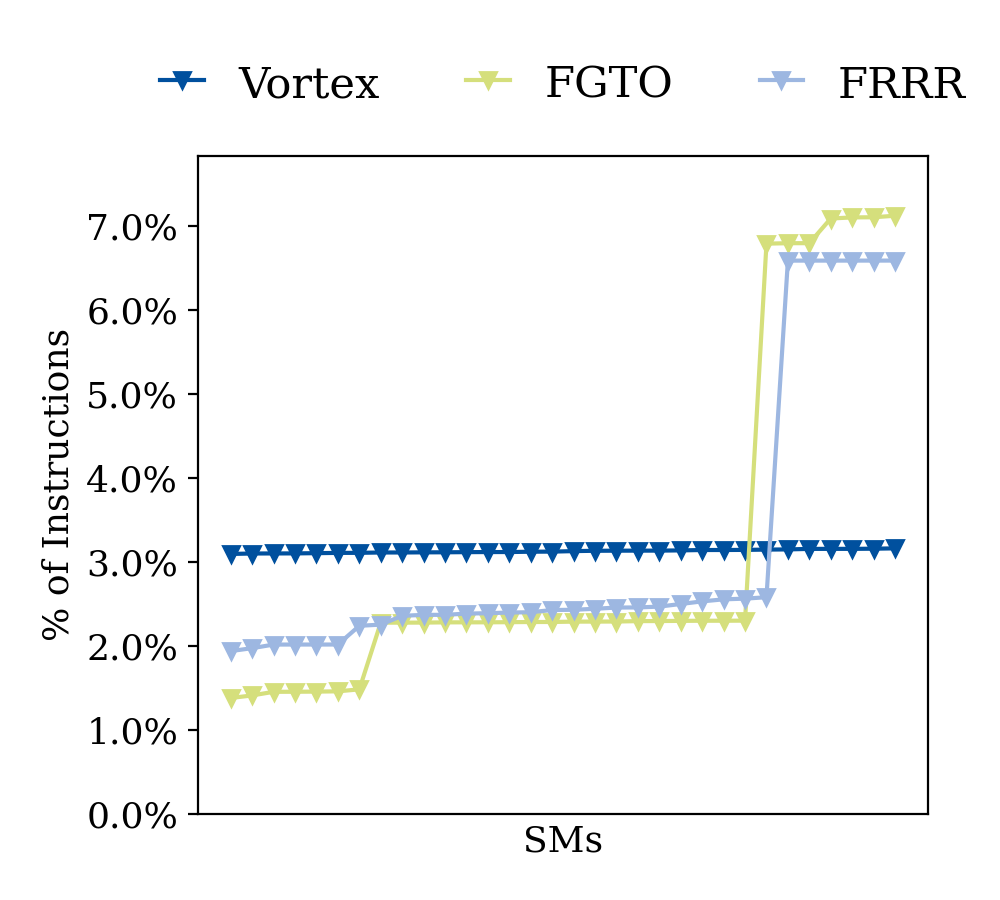
\includegraphics[width=\textwidth]{figures/instruction_distribution/nw_L2.png}
         \caption{NW}
         \label{fig:instr_dist_nw}
     \end{subfigure}
          \hfill
          \begin{subfigure}[t]{0.3\textwidth}
         \centering
         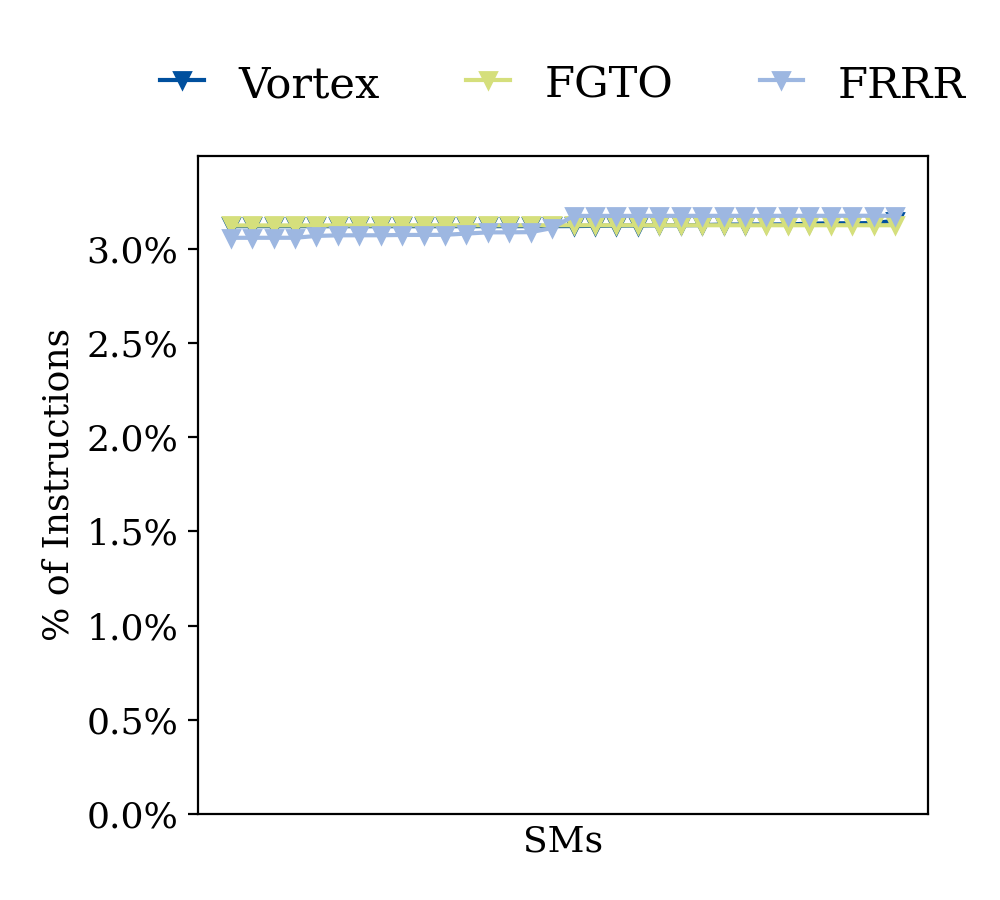
\includegraphics[width=\textwidth]{figures/instruction_distribution/psort_L2.png}
         \caption{Psort}
         \label{fig:instr_dist_psort}
     \end{subfigure}
          \hfill
          \begin{subfigure}[t]{0.3\textwidth}
         \centering
         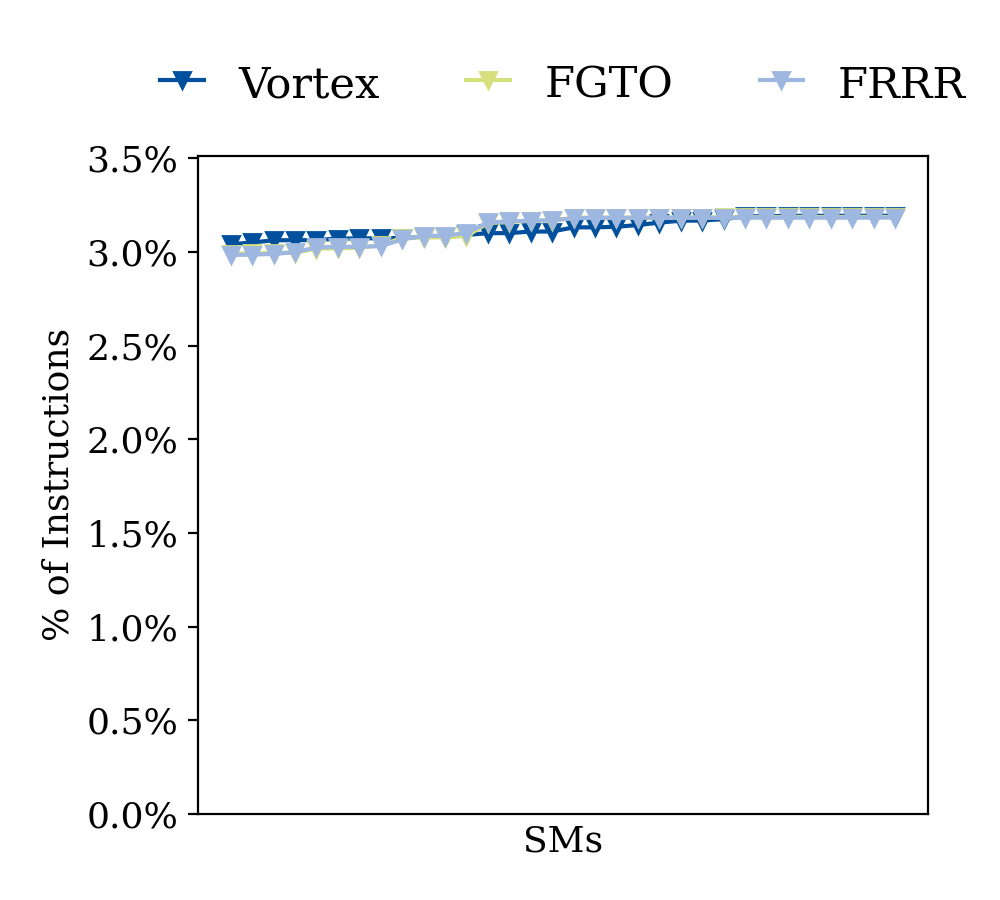
\includegraphics[width=\textwidth]{figures/instruction_distribution/saxpy_L2.png}
         \caption{SAXPY}
         \label{fig:instr_dist_saxpy}
     \end{subfigure}
          \hfill
          \begin{subfigure}[t]{0.3\textwidth}
         \centering
         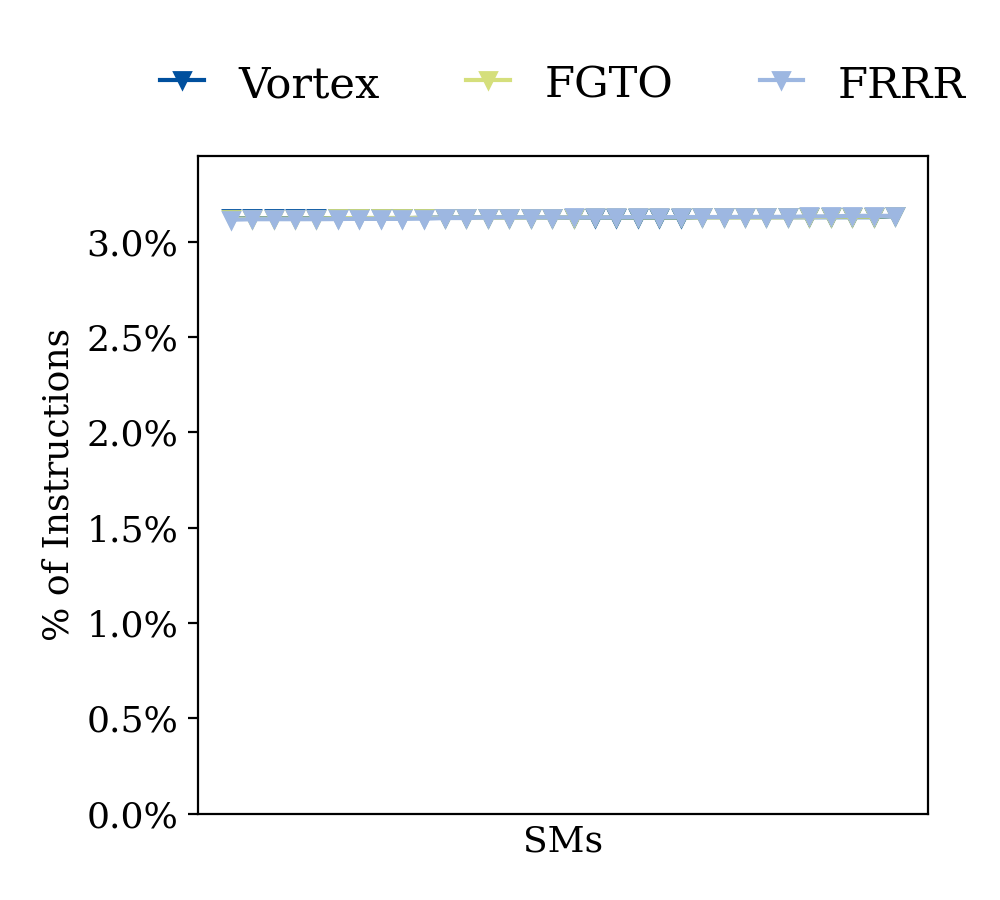
\includegraphics[width=\textwidth]{figures/instruction_distribution/sfilter_L2.png}
         \caption{Sfilter}
         \label{fig:instr_dist_sfilter}
     \end{subfigure}
     \hfill
     }

     \makebox[\linewidth][c]{
     \hfill
          \begin{subfigure}[t]{0.3\textwidth}
         \centering
         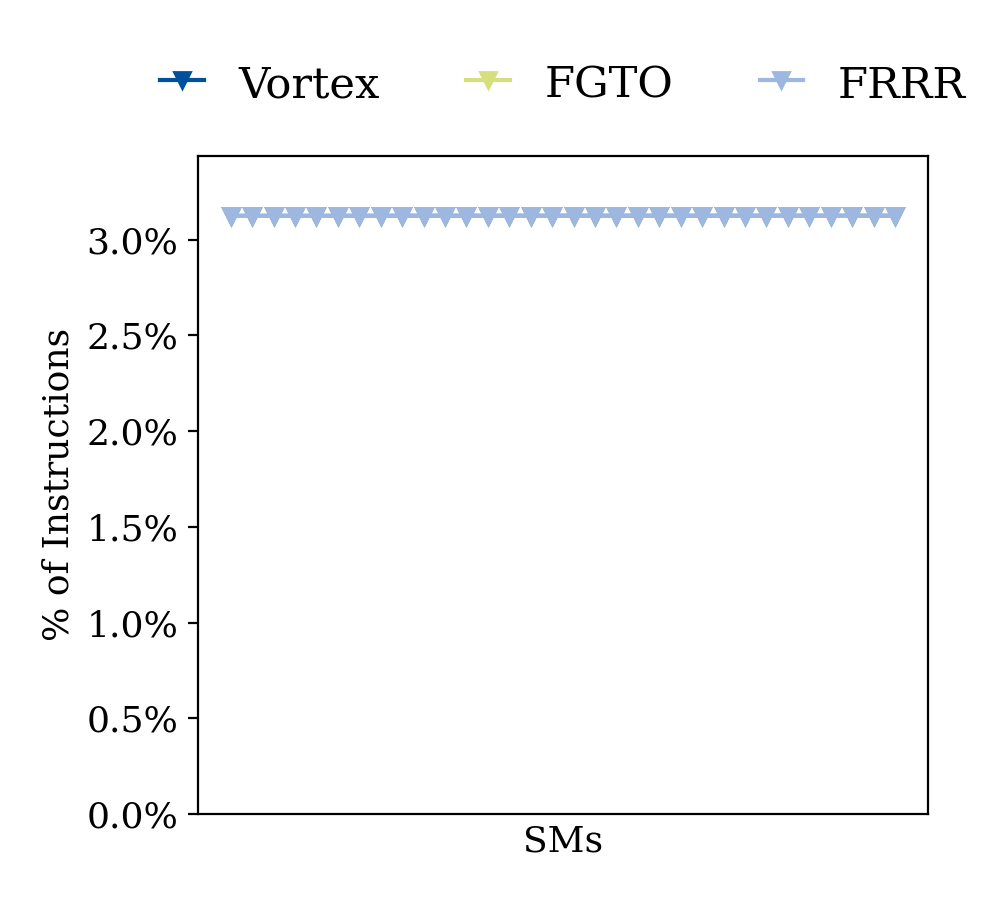
\includegraphics[width=\textwidth]{figures/instruction_distribution/sgemm_L2.png}
         \caption{SGEMM}
         \label{fig:instr_dist_sgemm}
     \end{subfigure}
          \hfill
     %      \begin{subfigure}[t]{0.3\textwidth}
     %     \centering
     %     \includegraphics[width=\textwidth]{figures/instruction_distribution/srad_L2.png}
     %     \caption{Srad}
     %     \label{fig:instr_dist_srad}
     % \end{subfigure}
          % \hfill
          \begin{subfigure}[t]{0.3\textwidth}
         \centering
         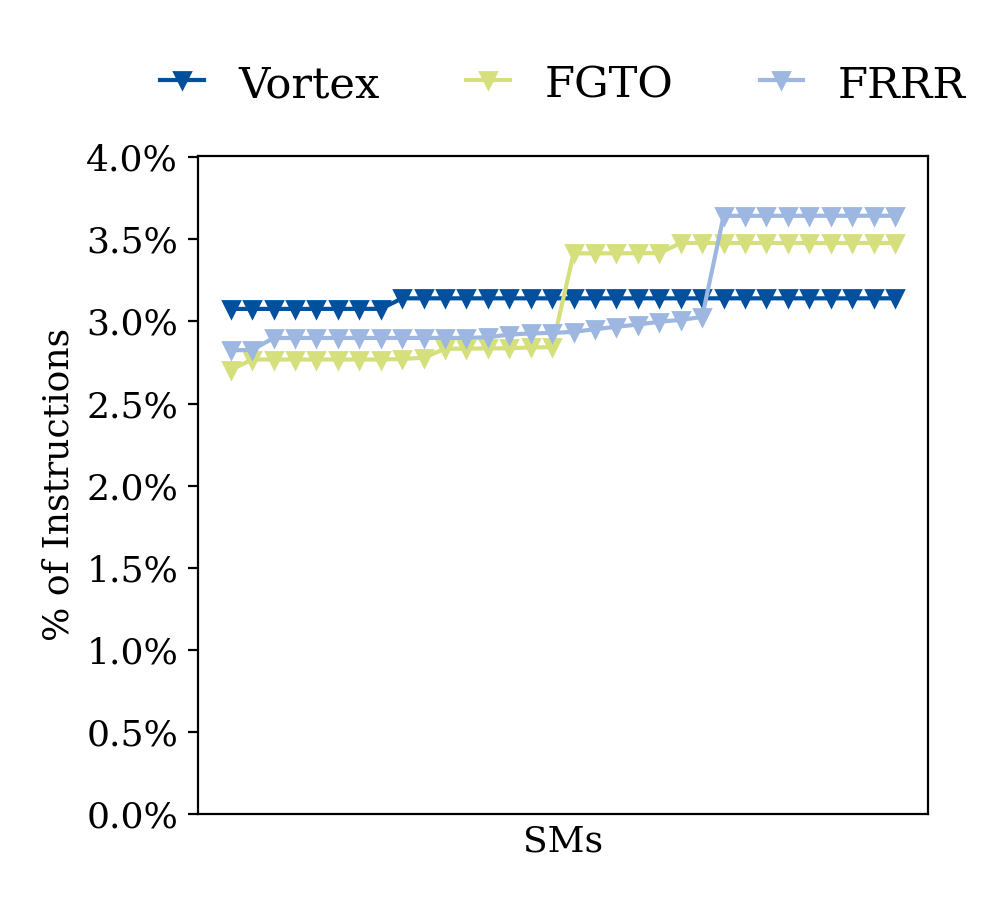
\includegraphics[width=\textwidth]{figures/instruction_distribution/streamcluster_L2.png}
         \caption{SC}
         \label{fig:instr_dist_streamcluster}
     \end{subfigure}
          \hfill
          \begin{subfigure}[t]{0.3\textwidth}
         \centering
         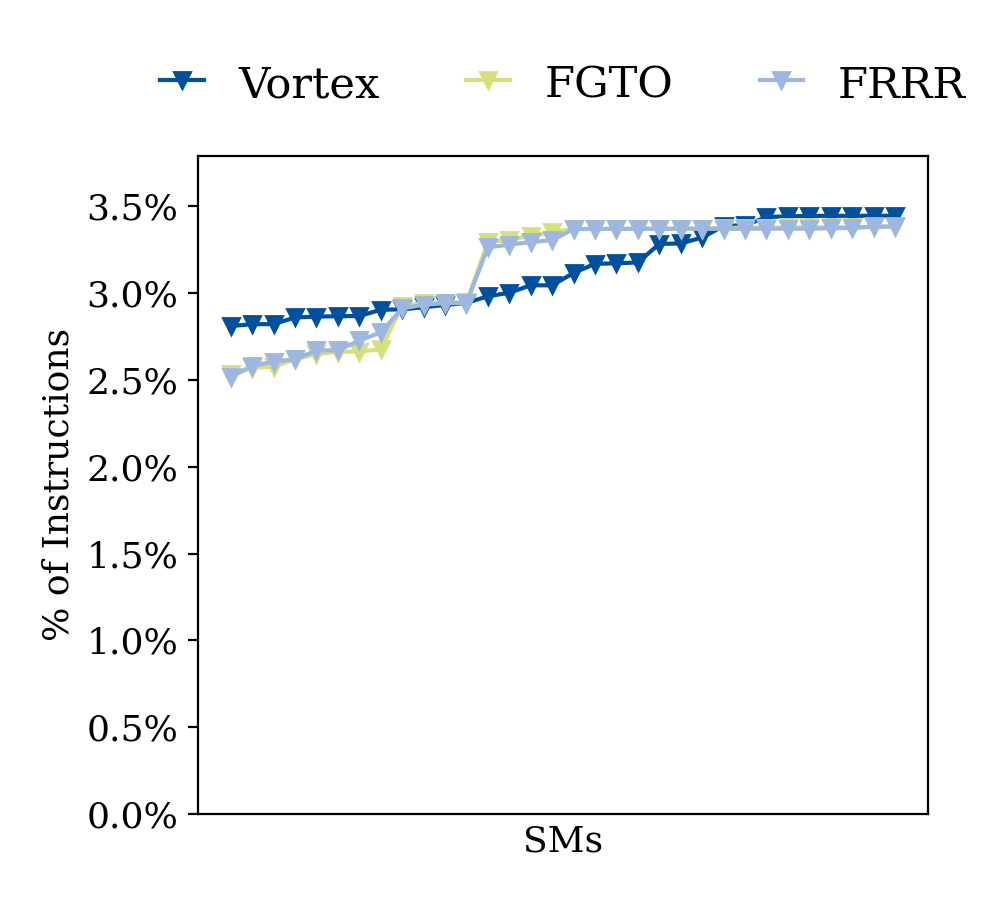
\includegraphics[width=\textwidth]{figures/instruction_distribution/vecadd_L2.png}
         \caption{Vecadd}
         \label{fig:instr_dist_vecadd}
     \end{subfigure}
     }

\caption[Distribution of executed instructions per \acrshort{sm}.]{Distribution of executed instructions per \acrshort{sm} for each of the benchmarks. The \acrshortpl{sm} are sorted in ascending order of their share of the executed instructions}
\label{fig:instruction_distribution}
\end{figure}

\begin{figure}
    \centering
    \makebox[\textwidth][c]{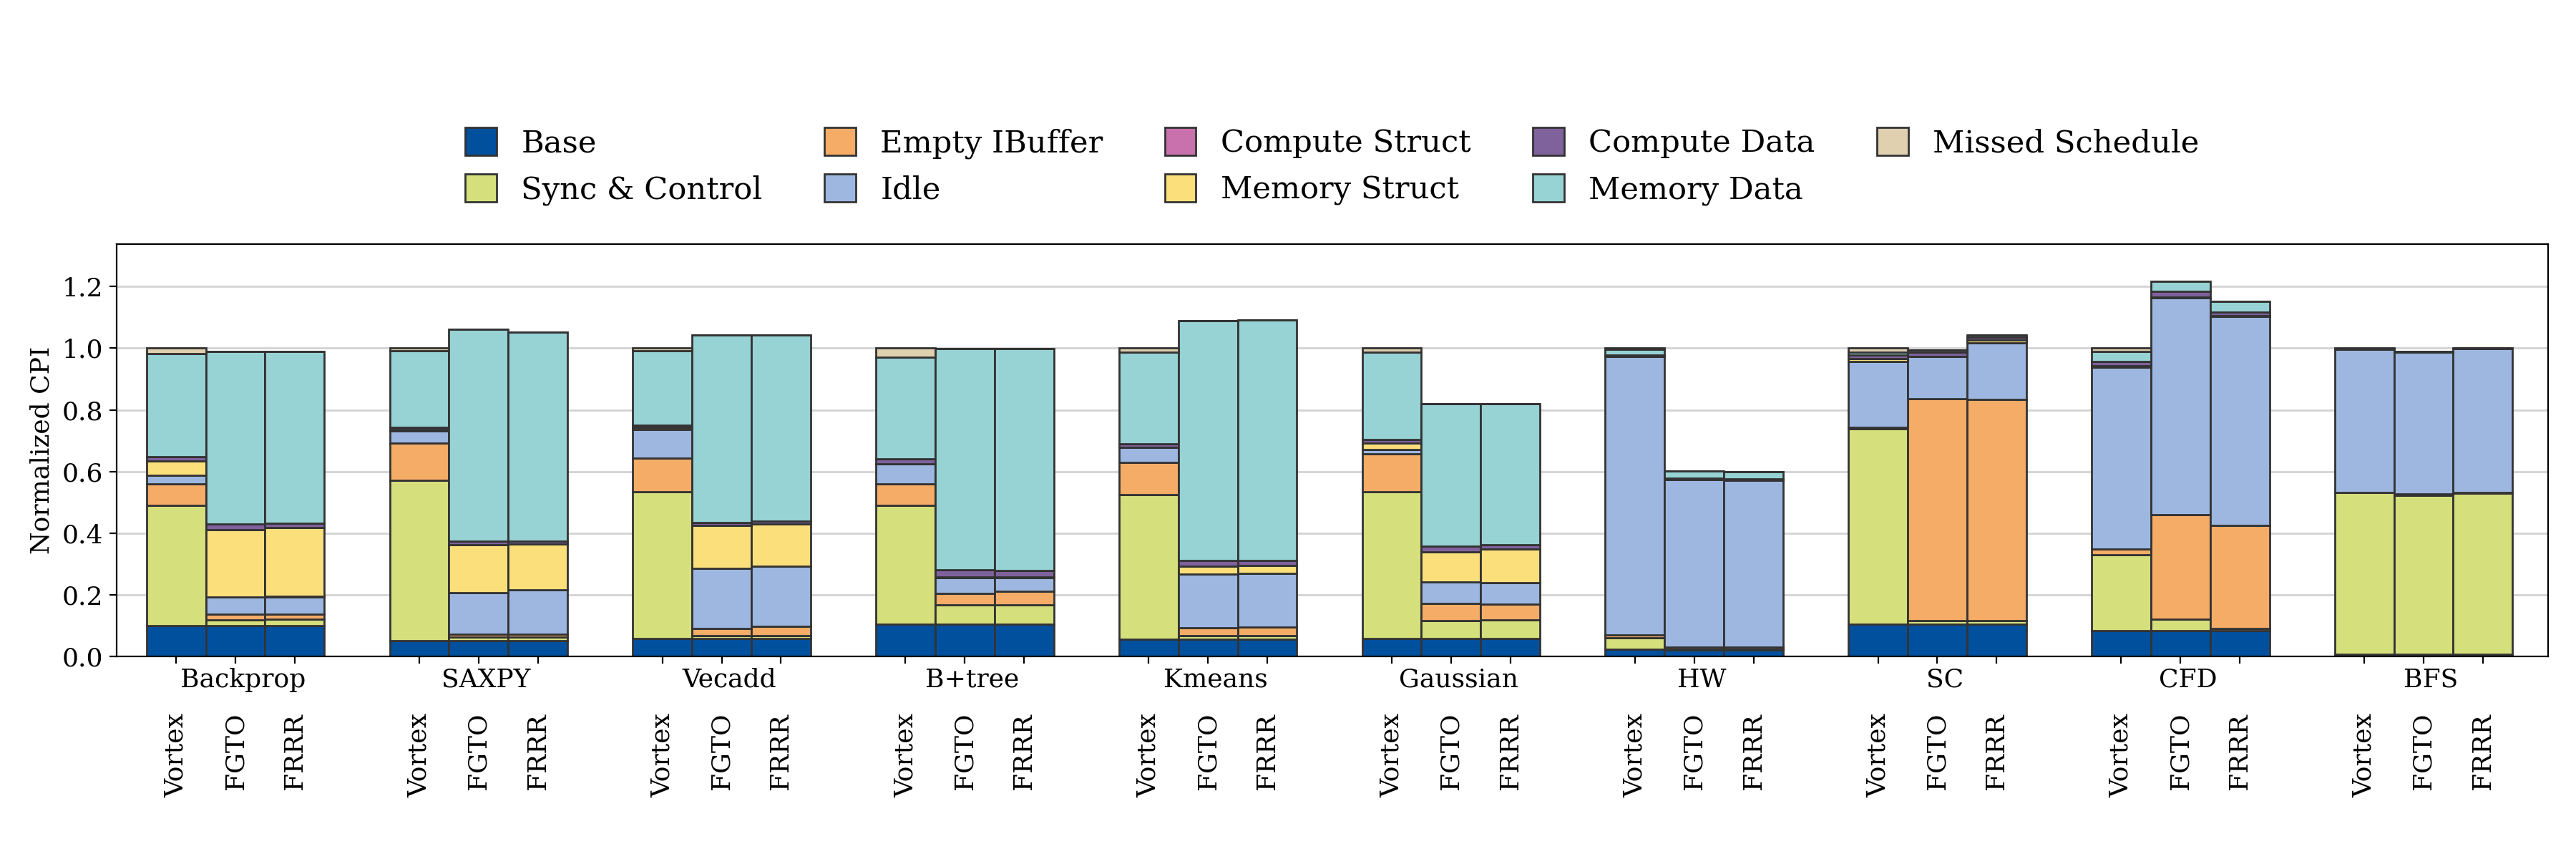
\includegraphics[width=1.3\textwidth]{figures/cpi_norm/L2_idle.png}}
    \caption{Normalized \acrshort{cpi} stacks for benchmarks with idle cycles}
    \label{fig:norm_cpi_idle}
\end{figure}

\textit{Backprop, saxpy, vecadd, b+tree, kmeans} and \textit{gaussian} all gain a significant number of idle cycles on \textit{FGTO} and \textit{FRRR}, as shown in Figure \ref{fig:norm_cpi_idle}. All of these benchmarks either finish execution, or complete multiple kernels before exiting early. The effects of uneven memory bandwidth distribution can thus be observed as idle cycles. As described in Section \ref{sec:results_memory}, the \acrshort{noc} is distributing the available bandwidth unfairly. This makes some \acrshortpl{sm} have higher throughput than others. As the \acrshortpl{tb} are statically distributed at the beginning of the kernel, the throughput difference will cause some of the \acrshortpl{sm} to finish earlier than others. The \acrshortpl{sm} will then have to idle until the kernel has finished execution. This is why the average bandwidth becomes lower for these benchmarks after implementing the changes. The skew in throughput cannot necessarily be observed in Figure \ref{fig:instruction_distribution} as these benchmarks finish execution, which levels out the number of executed instructions by \acrshortpl{sm} idling.

For the benchmarks which do not complete any kernels, the skewed memory bandwidth can be observed in the distribution of executed instructions. Because the kernels do not complete, the \acrshortpl{sm} are not idling, which is why it cannot be observed as idle stalls. Looking at \textit{hotspot} (Figure \ref{fig:instr_dist_hotspot}), \textit{DWT2D} (Figure \ref{fig:instr_dist_dwt2d}), \textit{lavaMD} (Figure \ref{fig:instr_dist_lavaMD}) and \textit{NW} (Figure \ref{fig:instr_dist_nw}), the difference between the \acrshortpl{sm} executing the most and least instructions is increased for \textit{FGTO} and \textit{FRRR} compared to \textit{\Gls{vortex}}. This is because \textit{FGTO} and \textit{FRRR} allow the \acrshortpl{sm} to issue more instructions, but the \acrshort{gpu} is throttled by the \acrshort{noc}, which is why there are only small improvements in performance. 

For benchmarks such as \textit{SC, CFD, HW} and \textit{BFS}, the proportion of idle cycles stays mostly the same for all three configurations. These idle cycles are caused by the \acrshort{tb} scheduler not being able to distribute workload to all of the \acrshortpl{sm}. This is apparent in Figure \ref{fig:instr_dist_bfs}, \ref{fig:instr_dist_cfd}, \ref{fig:instr_dist_hw} and \ref{fig:instr_dist_streamcluster}, where most of the \acrshortpl{sm} are not executing any instructions. I attempted to solve this by altering the local and global work sizes. This did however not affect the workload distribution. A better understanding of the \acrshort{tb} scheduler is probably required to solve this. 

In Figure \ref{fig:norm_cpi_idle}, the \acrshort{cpi} of \textit{HW} is almost halved for \textit{FGTO} and \textit{FRRR}. It appears as if the improvements are a result of a reduction in idle cycles. However, as shown in Figure \ref{fig:instr_dist_hw}, the same number of \acrshortpl{sm} continue to idle. Because of low memory contention, and the increased frontend and issue bandwidth, the performance of the active \acrshortpl{sm} improve drastically. The appearance of reduced idle cycles is thus caused by an increase in executed instructions by the active \acrshortpl{sm}, which in turn reduces the number of idle cycles per instruction.

\section{Warp Scheduling} \label{sec:results_warp_scheduling}

\begin{figure}
    \centering
    \makebox[\textwidth][c]{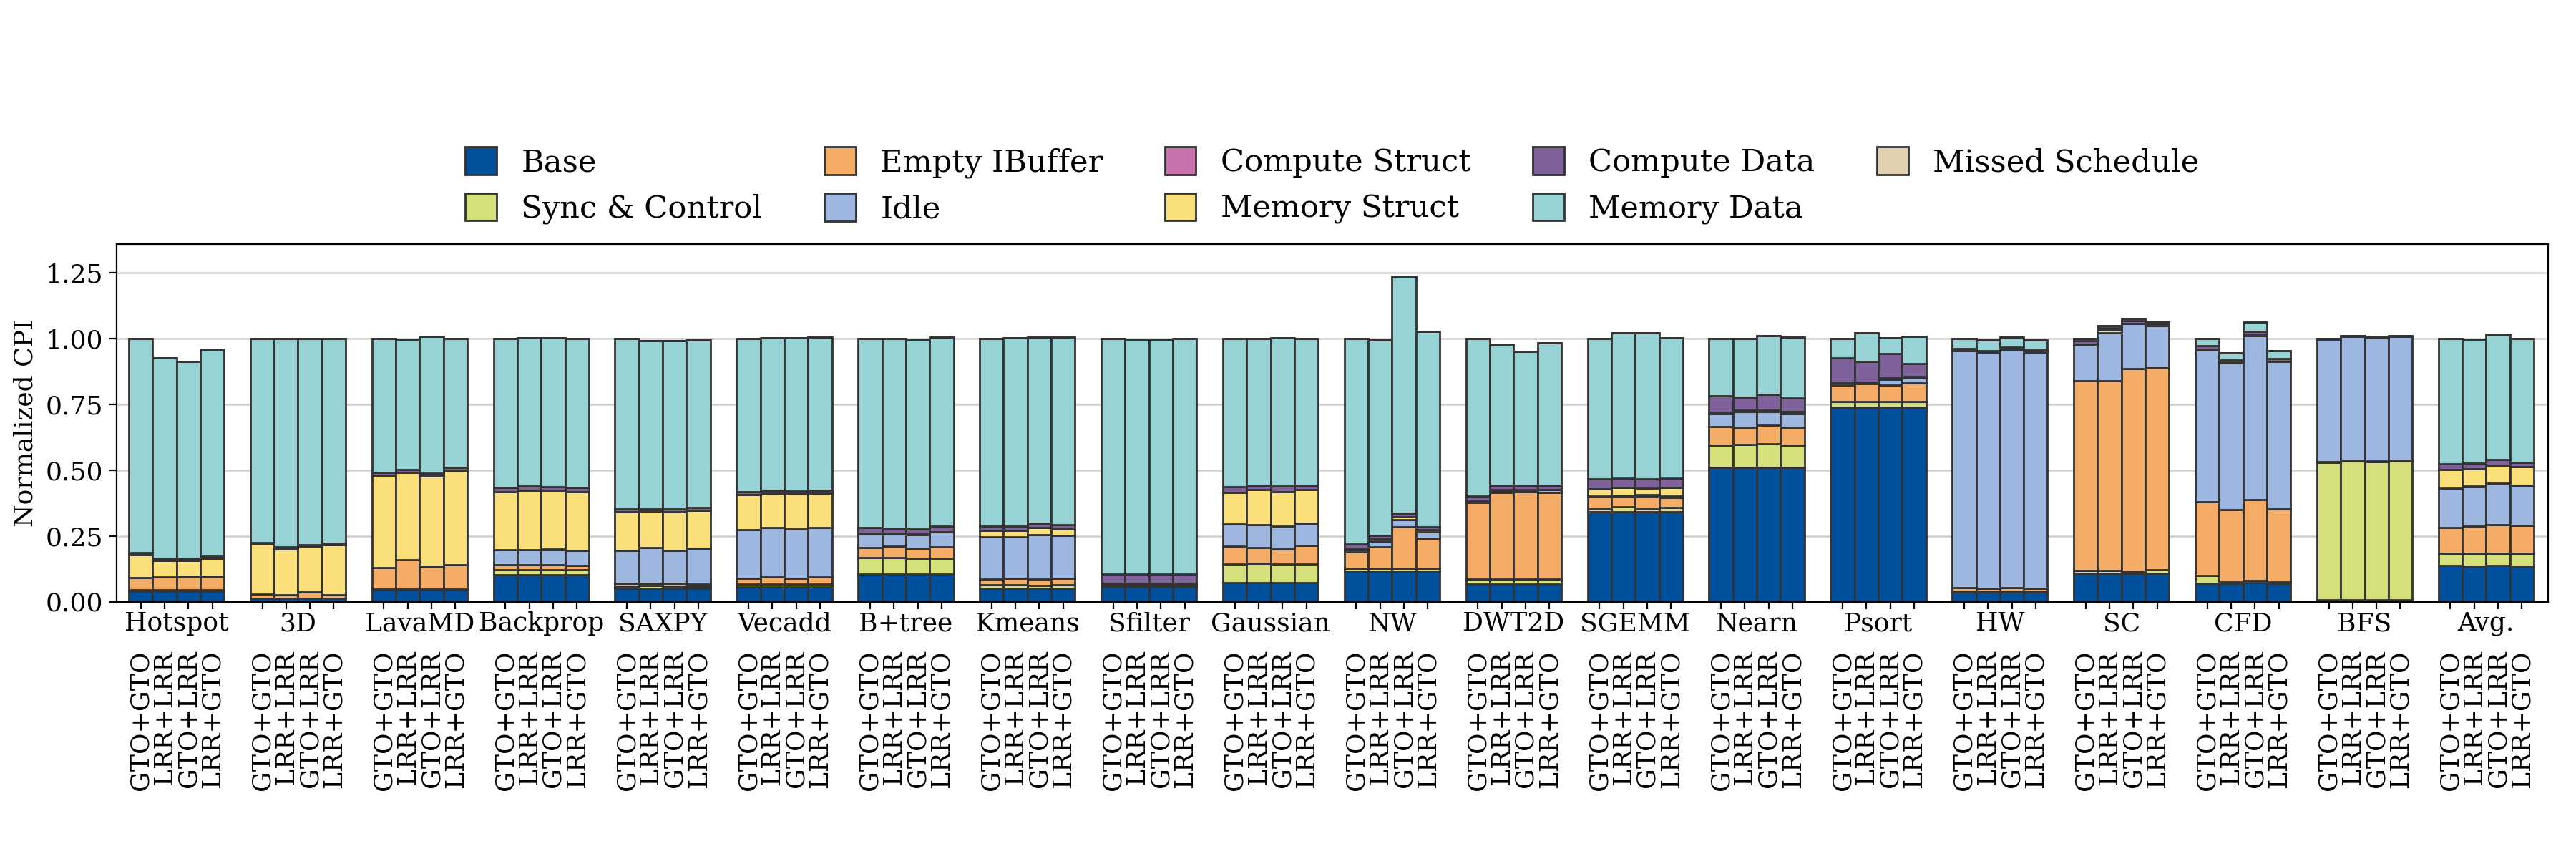
\includegraphics[width=1.3\textwidth]{figures/cpi_norm/Schedulers.png}}
    \caption[Normalized \acrshort{cpi} stacks comparing schedulers.]{Comparing combinations of scheduling algorithms used in the issue stage and fetch stage.}
    \label{fig:cpi_norm_schedulers}
\end{figure}

The motivation for implementing new schedulers for \Gls{vortex}, was to improve performance over the existing find-first and \acrshort{lrr} algorithms. In this section, I will compare combinations of the \acrshort{gto} and \acrshort{lrr} algorithms in the instruction and warp schedulers. The configurations will be described as \textit{fetch-algorithm}+\textit{issue-algorithm}. All of the configurations discussed in this section implement all the frontend improvements as well as ready scheduling.

For most of the benchmarks shown in Figure~\ref{fig:cpi_norm_schedulers}, the scheduling algorithm does not make a large difference. Looking at the average \acrshort{cpi}, the performance seems to be somewhat worse for \textit{GTO+LRR}, but the average \acrshort{cpi} stays within $1.5\%$ for all the other configurations. Most of the average \acrshort{cpi} increase for \textit{GTO+LRR} is coming from \textit{NW}. It is difficult to pinpoint an exact reason for this being an outlier. For \textit{CFD}, the performance is somewhat better when using a round-robin warp scheduler. This is because it has a large number of \textit{empty ibuffer} stalls. A round-robin warp scheduler will be able to fetch warps from different \acrshortpl{tb}, reducing the number of empty ibuffers, and thus reducing \textit{empty ibuffer} stalls. On the other hand, a \acrshort{gto} warp scheduler will attempt to fetch multiple warps from a single \acrshort{tb}, and thus only fill one ibuffer. If a warp fetched by \acrshort{gto} cannot be issued, it is therefore less likely to be other warps available in the instruction buffer to hide the stall.

The motivation for using \acrshort{gto} was to improve cache usage and reach long-latency stalls earlier. This is clearly not happening, since there is no significant difference in the number of \textit{memory data} stalls between the configurations. There are multiple possible reasons why the \acrshort{gto} scheduler might not perform as expected:

\begin{itemize}
    \item The current implementation of \acrshort{gto} does not differentiate between long- and short-latency stalls. If a warp is stalled due to a short-latency stall, e.g. a cache hit, its age is set to 0. Thus it will become a low-priority warp before it hits a long-latency stall. This might also lose potential cache hits, as the \acrshort{gto} scheduler will then begin to schedule other warps, which can evict cache-lines used by the short-latency stalled warp. Setting the age of the warp to 0 only upon detecting long-latency stalls would allow the warp to keep high priority and hit long-latency stalls sooner. This might improve cache usage and reduce the number of stall cycles due to long-latency memory requests. 
    \item The interaction between the warp scheduler, issue scheduler and \acrshort{bpr} might not be ideal for \acrshort{gto}. To get the most out of \acrshort{gto} scheduling, it should be able to consecutively issue as many warps from the same \acrshort{tb} as possible. If the currently selected greedy warp ID of the two schedulers are different, i.e. they schedule warps from different \acrshortpl{tb}, the instruction buffer might empty before hitting the desired long-latency stall. \acrshort{bpr} forces the warp scheduler to fetch warps from a different \acrshort{tb} if the instruction buffer is full. This can prevent the warp scheduler from fetching enough instructions to hit long-latency stalls. A solution to this would be to increase the queue size of the instruction buffer.  
    \item With only 4 \acrshortpl{tb} per \acrshort{sm}, there might be too few warps to be able to hide any significant number of long-latency stall cycles.
\end{itemize}

% - too few warps to hide stalls in a significant manner
% - bad interaction with the gto warp scheduler and gto issue scheduler
% - short latency stalls stop gto from prioritizing the \acrshort{tb} until it hits a long latency stall 

% \section{Implementation cost}

% \textcolor{red}{Each of the configuration has an associated area cost and critical path which controls the maximum frequency of the GPU. Following is a plot of the total area and critical paths}

\section{Sensitivity Analysis}

I performed various sensitivity analyses based on the memory bandwidth, the number of warps per \acrshort{sm} and the caches. The goal is to see how these factors affect \textit{FGTO} and \textit{FRRR} compared to \textit{\Gls{vortex}}, not necessarily how they affect the overall performance.

\begin{figure}
    \centering
    \makebox[\textwidth][c]{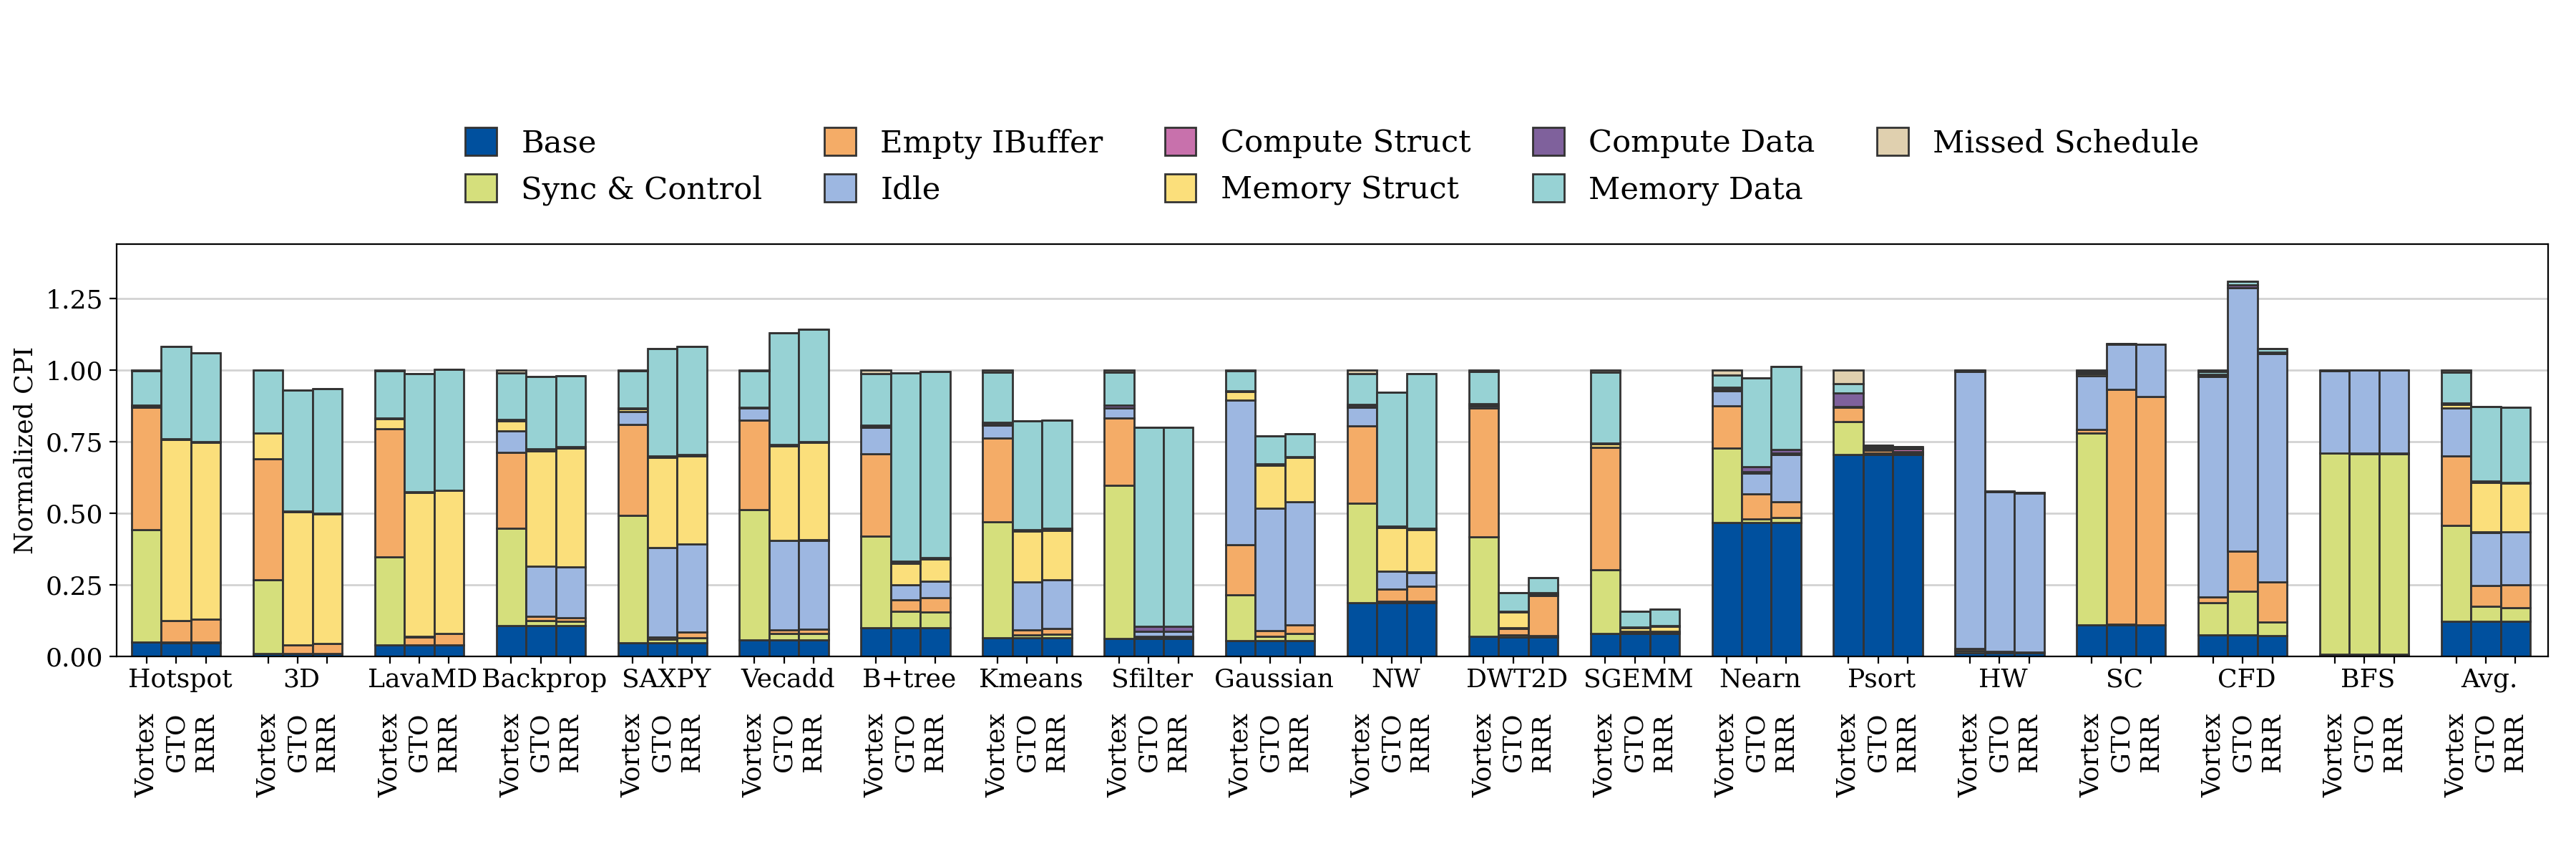
\includegraphics[width=1.3\textwidth]{figures/cpi_norm/L2_8W.png}}
    \caption[Normalized \acrshort{cpi} stacks when using 8 warps per \acrshort{sm}.]{Normalized \acrshort{cpi} stacks for the baseline and final versions using 8 warps per SM}
    \label{fig:norm_cpi_8w}
\end{figure}

\vspace{1mm}\noindent
\textbf{Increase warps per \acrshort{sm}}. Figure~\ref{fig:norm_cpi_8w} shows the \acrshort{cpi} stacks for the same configuration as described in the experimental setup but with 8 warps per \acrshort{sm}. On average \textit{FGTO} and \textit{FRRR} respectively reduce \acrshort{cpi} by $12.9\%$ and $13.2\%$ over \textit{\Gls{vortex}}. This is a greater reduction than when using 4 warps per \acrshort{sm}. When using 8 warps per \acrshort{sm}, a larger proportion of the stalls in \textit{\Gls{vortex}} are frontend stalls. The baseline configuration thus continues to be inhibited by the frontend throughput. The increase is mainly due to the increase in \textit{empty ibuffer} stalls. This is because the frontend is unable to fetch enough instructions to fill the increased number of instruction buffers. The \textit{FGTO} and \textit{FRRR} are clearly still able to fill the instruction buffer, as there are close to no frontend stalls in any of the benchmarks. \textit{SRAD, SC, BFS} and \textit{CFD} continue to experience the same issues as described in Section \ref{sec:result_control_stalls}. 

The increased frontend throughput allows \textit{FGTO} and \textit{FRRR} to utilize memory bandwidth and hide data stalls to a greater degree, as shown by the increased proportion of \textit{memory structural} stalls. The \acrshort{cpi} of \textit{sgemm} is reduced to a much larger degree by \textit{FGTO} and \textit{FRRR} when using 8 warps than when using 4 warps. When using 4 warps, \textit{sgemm} is largely dominated by \textit{memory data} stalls. By increasing the number of warps to 8, the low average latency of \textit{sgemm} can be hidden, resulting in a drastic performance improvement. The same goes for \textit{psort} which is close to never stalling for both \textit{FGTO} and \textit{FRRR}.

The increased \acrshort{mlp} caused by having more warps, is increasing the memory bandwidth requirement. Because of this, the \acrshort{noc}'s skewed bandwidth distribution is likely to have an even greater effect. This is why benchmarks such as \textit{vecadd} are seeing a larger proportion of \textit{idle} stalls. For \textit{gaussian}, the increased proportion of \textit{idle} stalls is likely a combination of skewed bandwidth distribution and the workload not being divided into enough \acrshortpl{tb} to fill the increased number of \acrshort{tb} slots per \acrshort{sm}.   

\begin{figure}
    \centering
    \makebox[\textwidth][c]{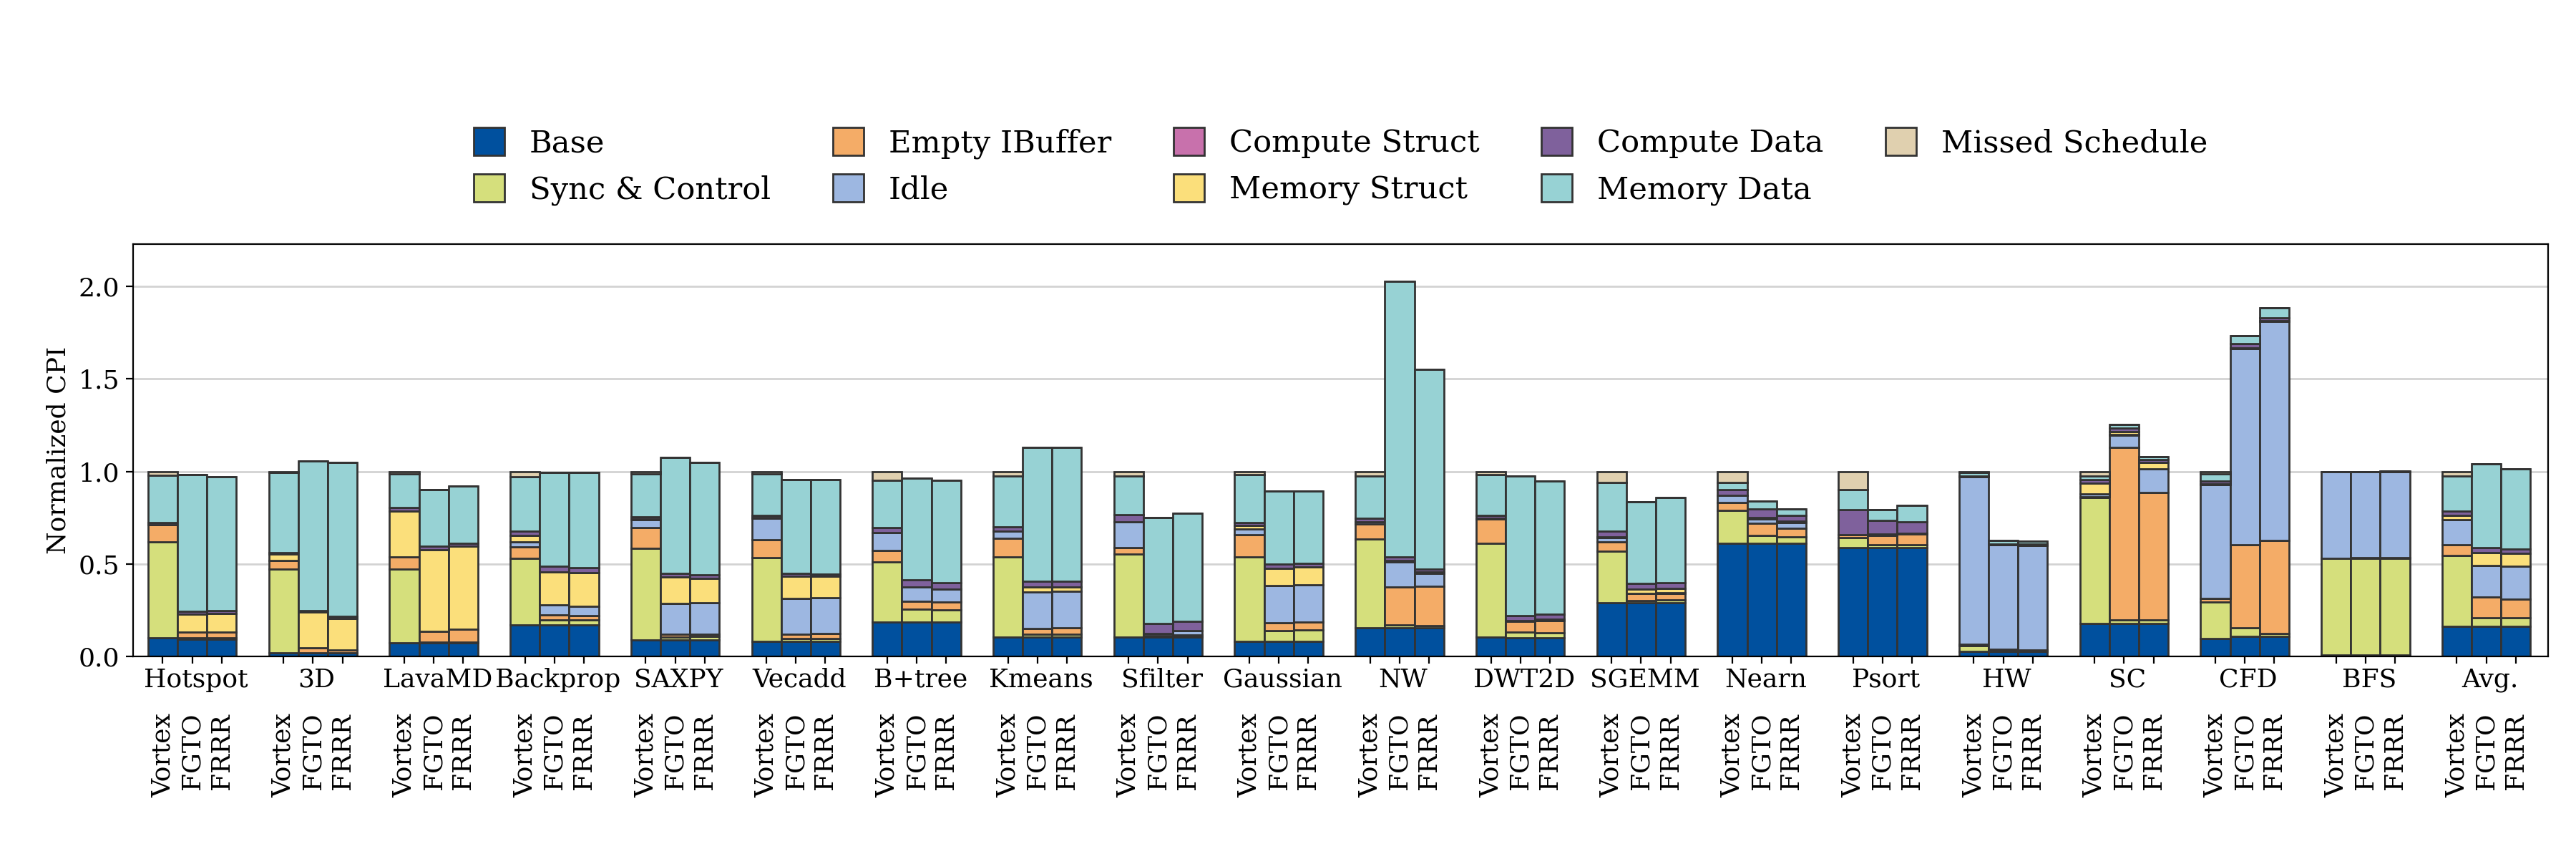
\includegraphics[width=1.3\textwidth]{figures/cpi_norm/L2_2channel_ddr4.png}}
    \caption[Normalized \acrshort{cpi} stacks with double the available memory bandwidth]{Normalized CPI stacks when using two memory channels, giving a bandwidth of $34.8GB/s$}
    \label{fig:2channel_memory}
\end{figure}

\vspace{1mm}\noindent
\textbf{Increase DDR4 bandwidth.} Figure \ref{fig:2channel_memory} shows the \acrshort{cpi} stacks for \Gls{vortex} using 2 channel DDR4 memory, resulting in $34.8GB/s$ of bandwidth, giving $2\times$ the available bandwidth of the memory configuration described in the experimental setup. For benchmarks with high bandwidth utilization, such as \textit{lavaMD}, the additional available bandwidth enables both \textit{FGTO} and \textit{FRRR} to reduce \acrshort{cpi}, instead of increasing it. For most other benchmarks, the additional memory bandwidth does not alter how the changes affect \acrshort{cpi}. The benchmarks continue to be dominated by \textit{memory data} stalls, and are thus unable to utilize the bandwidth. Thus both \textit{FGTO} and \textit{FRRR} remain latency bound. It is difficult to determine why the \acrshort{cpi} of \textit{NW} and \textit{CFD} for are almost doubled for \textit{FGTO} and \textit{FRRR} compared to \textit{\Gls{vortex}}. I believe it might be an issue with the simulation, as I previously experienced issues, where the simulator gave erroneous results.

\newpage
\vspace{1mm}\noindent
\textbf{Only L1 caches.} Figure \ref{fig:norm_cpi_L1} shows the normalized \acrshort{cpi} stacks when using only L1 caches, i.e. not using a L2 cache for each cluster. For most of the benchmarks, the increased memory latency of having no L2 cache makes \textit{FGTO} and \textit{FRRR} have less impact on performance as a smaller proportion of the stall cycles can be hidden. Most interestingly, the \textit{idle} stalls incurred by skewed bandwidth distribution in \textit{backprop, saxpy, vecadd, b+tree, kmeans and gaussian} are gone. This indicates that the L2 cache bandwidth might be too low, or  the memory arbiters replacing the L2 caches, are distributing the memory bandwidth differently. Interestingly \textit{FGTO} and \textit{FRRR} reduce \acrshort{cpi} by $7.02\%$ and $7.42\%$ respectively, which is more than when using L2 caches. The extra improvement mostly comes from there being no additional idle stalls. 

The \acrshort{cpi} is drastically increased for \textit{NW} in the \textit{FGTO} and \textit{FRRR} configurations. This increase is due to a large increase in \textit{memory data} stalls. The increased frontend throughput might cause the requests to queue up in the memory system, as described in Section~\ref{sec:results_memory}. This effect becomes even stronger as the L1 cache hit rate is low and the L2 cache is removed. Because of this, the latency is increased which in turn increases \textit{memory data} stalls.

\begin{figure}
    \centering
    \makebox[\textwidth][c]{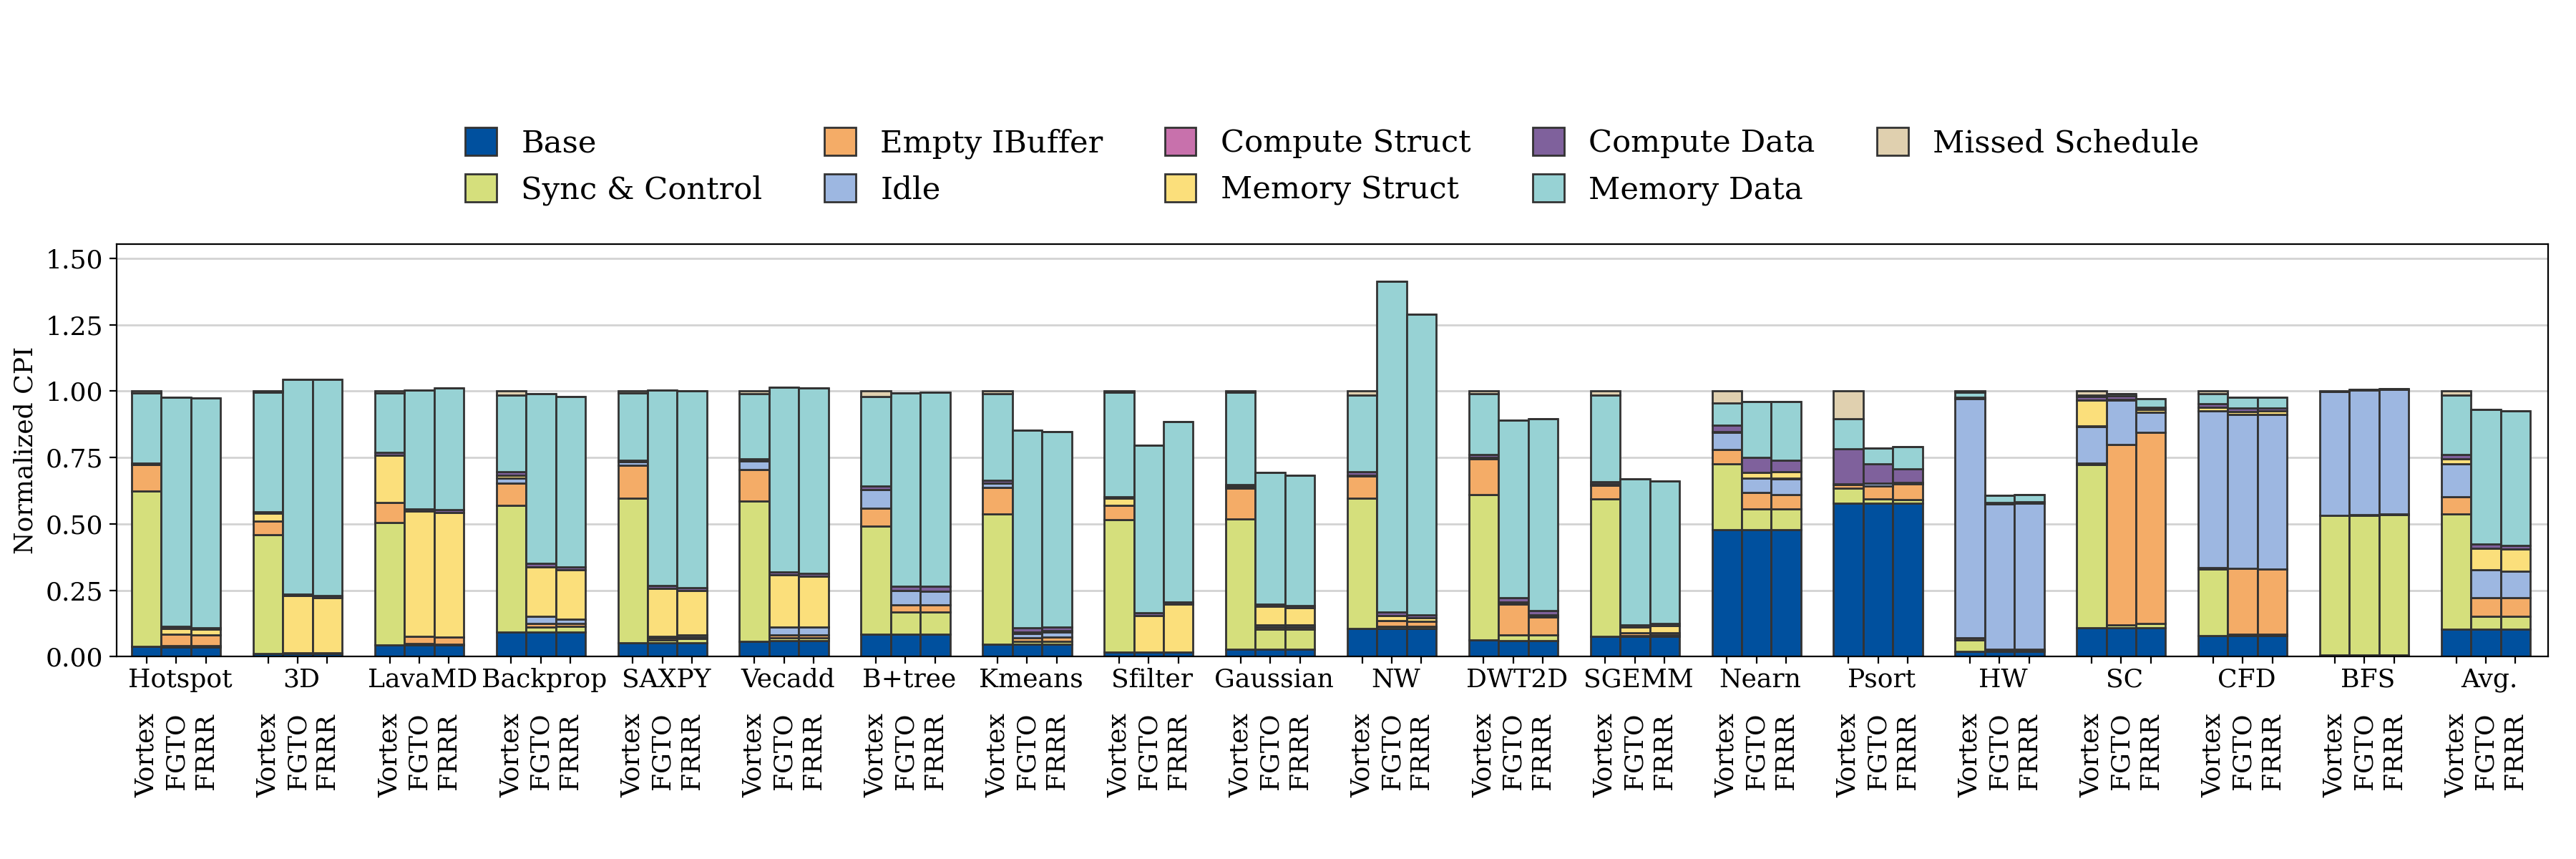
\includegraphics[width=1.3\textwidth]{figures/cpi_norm/L1.png}}
    \caption{Normalized CPI stacks when using only L1 caches}
    \label{fig:norm_cpi_L1}
\end{figure}